\documentclass[10pt]{article}
\usepackage{ctex}
\usepackage{makecell} %单元格内换行

\usepackage{amsmath,mathrsfs,amsfonts} %公式手动编码不能再 $ $$中
\usepackage{yhmath}%AB弧
\usepackage{tikz}
\usepackage{calc}
\usepackage{graphicx}
%\usepackage{pgfplots}

\usepackage{amssymb}
\usepackage{cases}  %方程组每一个都编码
\usepackage{sectsty} % 引入sectsty包 设置section字体大小
\usepackage{pifont}
\sectionfont{\fontsize{11}{12}\selectfont\centering}% 设置section的字体大小
\subsectionfont{\fontsize{11}{12}\selectfont}% 设置section的字体大小

% 设置页面的环境,a4纸张大小,左右上下边距信息
\usepackage[a5paper,left=5mm,right=5mm,top=14mm,bottom=5mm]{geometry}
\usepackage{fancyref}
%\usepackage{graphicx}
% 使用indentfirst宏包
\usepackage{indentfirst}
% 设置首行缩进距离
\setlength{\parindent}{0em}


%\centering %居中
\headsep=2mm


\usepackage{fancyhdr}

\begin{document}
%hello latex
%\large hello latex
%\Large %hello latex
%\LARGE hello latex
%\huge hello latex
%\Huge hello latex

\title{争取未来开挖掘机} %文章标题
\author{姜圣的追随者}  %作者
\date{2024.7.12} %当天时间

\maketitle %添加这一句才能够显示标题等信息
\newpage
\begin{abstract}
    沉迷游戏的我无意间看见关于姜圣的新闻。深感愧疚,幼儿班的我就已经熟练的掌握了的九九乘法表。而现在我却每天沉迷于提瓦特大陆,天天只知道打丘丘人。\par 从今天开始我也要努力学习数学,希望姜圣以后当上院士的时候能带我一起开发挖掘机。
    \\(本书内容:仅有公式,定理及证明)
    \\(作者文凭:中专学历,混的文凭,简单理解就是初中学历(-。- )!)
    \\(公式及证明出处:公式及证明都是在别的书里参考过来的,极个别公式证明是我自己瞎写的。)
    \\本书的pdf,及latex源码地址:https://github.com/daidongchuixue/jiangping.git
    \\2024.7.31:本书几乎是跟着B站高数视频记录的。记录完,会作为第一版。(预计时间几个月)然后参考数学分析书籍重新整理,为第二版。
    \\2024.8.5:联系方式,姜萍吧,姜圣的追随者,
\end{abstract}
\newpage
\renewcommand{\contentsname}{目录}
\tableofcontents %目录设置


\pagestyle{fancy} %页眉页脚
%\fancyhy{}
%\fancyhead{LE}{\rightmark}

\numberwithin{equation}{subsection}

\section{三角函数}
\subsection{三角恒等式}
\begin{align}
    \sin(A+B)= \sin A\cos B+\cos A\sin B\\
    \sin(A-B)= \sin A\cos B-\cos A\sin B\\
    \cos(A+B)= \cos A\cos B-\sin A\sin B\\
    \cos(A-B)= \cos A\cos B+\sin A\sin B
\end{align}
\subsubsection{和差化积}
\begin{align}
    \sin(\alpha)+\sin(\beta)=2\sin\left(\frac{\alpha+\beta}{2}\right)\cos\left(\frac{\alpha-\beta}{2}\right)\\
    \sin(\alpha)-\sin(\beta)=2\cos \left(\frac{\alpha+\beta}{2}\right)\sin\left(\frac{\alpha-\beta}{2}\right)\\
    \cos(\alpha)+\cos(\beta)=2\cos \left(\frac{\alpha+\beta}{2}\right)\cos\left(\frac{\alpha-\beta}{2}\right)\\
    \cos(\alpha)-\cos(\beta)=-2\sin \left(\frac{\alpha+\beta}{2}\right)\sin\left(\frac{\alpha-\beta}{2}\right)
\end{align}

\subsubsection{倍角公式}
\begin{displaymath}
    \centering
    \begin{split}
        \sin(2x)=2\sin x\cos x\\
        \cos(2x)=\cos^2x-\sin^2x=1-2\sin^2 x\\
        \tan(2x)=frac{2\tan x}{1-\tan^2x}
    \end{split}
\end{displaymath}
\subsection{双曲函数}
定义
$$\sinh x = \frac{e^x-e^{-x}}{2}\qquad \cosh x = \frac{e^x+e^{-x}}{2}$$
$$\tanh x = \frac{e^x-e^{-x}}{e^x+e^{-x}}\qquad \coth x = \frac{e^x+e^{-x}}{e^x-e^{-x}}$$
恒等式
\begin{align}
&\sinh (2x) = 2\sinh x\cosh x \label{eq:hyperbolic_functions_1} \\
&\cosh^2x-\sinh^2x = 1 \label{eq:hyperbolic_functions_2} \\
&\cosh^2x+\sinh^2x = cosh (2x) \label{eq:hyperbolic_functions_3} \\
&\cosh x = 1+2\sinh^2\frac{x}{2} \label{eq:hyperbolic_functions_4}
\end{align}
 %三角函数
\section{不等式}

\begin{align}
\frac{x_1+x_2+\dots+x_n}{n}\geqslant \sqrt[n]{x_1+x_2+\cdots+x_n}
\end{align}

\begin{align}
|x+y|<|x|+|y|
\end{align}

\begin{align}
\sin x < x < \tan x
\end{align}

伯努利不等式
\begin{align}
(1+x)^n\leqslant 1+nx
\end{align}
 %不等式
\section{排列组合}
\subsection{定义}
\begin{align}
\mathbb{A}_n^k &= \frac{n!}{(n-k)!}=n(n-1)(n-2)\cdots(n-k+1) \\
\mathbb{C}_n^k &= \frac{\mathbb{A}_n^k}{k!} = \frac{n!}{k!(n-k)!}=\frac{n(n-1)(n-2)\cdots(n-k+1)}{k!}
\end{align}
\subsection{运算}
 %排列组合
\section{区间与映射}
\subsection{区间定义}
区间定义$\begin{cases}
    (a,b)=\{x|a<x<b\} \\
[a,b]=\{x|a\leqslant x\leqslant b\}\\
(a,b]=\{x|a<x\leqslant b\} \\
(a,+\infty)=\{x|a<x\}
\end{cases}
$ \par
\subsection{领域定义}

点a的领域
\begin{figure}[htp]
   % \centering
    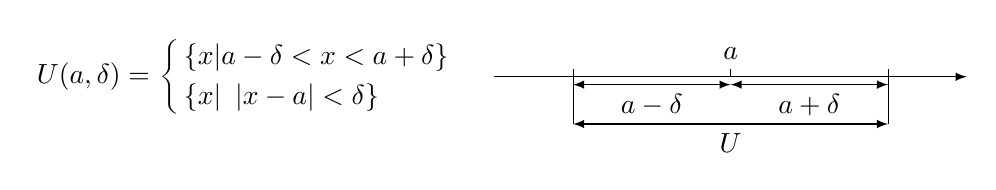
\begin{tikzpicture}[>=latex]
        \node at (-6,0){$U(a,\delta)=\begin{cases}
        \{x|a-\delta<x<a+\delta\}\\
        \{x|\ \left|x-a\right|<\delta\}
        \end{cases}$};
        \draw[->] (-3,0)--(3,0);
        \draw (0,0)--(0,.1);
        \foreach \x in {-2,2}
        {
            \draw (\x,-.6)--(\x,.1);
        }
        \draw[<->] (-2,-.6)--node[below]{$U$}(2,-.6);
        \node at (0,.1)[above]{$a$};
        \draw[<->] (-2,-.1)--node[below]{$a-\delta$}(0,-.1);
        \draw[<->] (0,-.1)--node[below]{$a+\delta$}(2,-.1);
    \end{tikzpicture}
    %\caption{asd}\label{dsa}
\end{figure}

点a的去心领域\par
\begin{figure}[htp]
    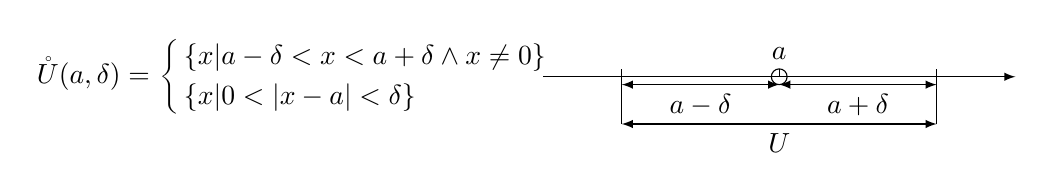
\begin{tikzpicture}[>=latex]
        \node at (-6,0){$\mathring{U}(a,\delta)=\begin{cases}
        \{x|a-\delta<x<a+\delta\land x\neq 0\}\\
        \{x|0<\left|x-a\right|<\delta\}
        \end{cases}$};
        \draw[->] (-3,0)--(3,0);
        \draw (0,0)--(0,.1);
        \foreach \x in {-2,2}
        {
            \draw (\x,-.6)--(\x,.1);
        }
        \draw[<->] (-2,-.6)--node[below]{$U$}(2,-.6);
        \node at (0,.1)[above]{$a$};
        \draw (0,0)circle(.1);
        \draw[<->] (-2,-.1)--node[below]{$a-\delta$}(0,-.1);
        \draw[<->] (0,-.1)--node[below]{$a+\delta$}(2,-.1);
    \end{tikzpicture}
\end{figure}
点a的左领域$\qquad(a-\delta,a)$\par
点a的右领域$\qquad(a,a+\delta)$
\subsection{映射定义}
定义:X与Y是两个非空集合,如果存在一个法则对任一$x\in X$, 都有确定的y与之对应。
则称f为从X到Y的一个映射。
$$\mbox{记作}\qquad f:X\rightarrow Y$$
$$f(x)=y\qquad\begin{cases}
    \mbox{定义域}\ (D_f)=X &x\mbox{-原像} \\
    \mbox{值域}\ (R_f)=\{f(x)|x\in X\} \qquad&y\mbox{-像}
\end{cases}$$
映射类型$\quad
\begin{cases}
    \mbox{满射:} &R_f = Y \\
    \mbox{单射:} &x_1\neq x_2\Rightarrow f(x_1)\neq f(x_2)\\
    \mbox{一一映射:}&\mbox{即使满射又是单射}\Leftrightarrow\mbox{逆映射:}
    \begin{cases}
        f^(x)&=y\\
        f^{-1}(y)&=x
    \end{cases}\\
    \mbox{复合映射:}&g\circ f\Leftrightarrow g\left[f\left(x\right)\right]
    \begin{cases}
        f:X\rightarrow Y_1\\
        g:Y_2\rightarrow Z\\
        g\circ f:X\rightarrow Z\qquad(Y_1 \subset Y_2)
    \end{cases}
    %\circ  
\end{cases}$%区间与映射
\section{函数与图像}
\subsection{函数的定义}
设数集$D\in R$的映射
$$f: D\rightarrow R$$
称f为定义在D上的函数,记为
$$y = f(x)\ \{x\in D\}$$
 \subsection{函数的性质}
 \subsubsection{函数的有界性}
 $f:D\rightarrow R\{D\subset R\}$$\begin{cases}
    \mbox{有界}\begin{cases}
        \mbox{有上界}\begin{cases}
            \exists k_1,\ \mbox{使}f(x)\leqslant k_1,\ \forall x\in D  
        \end{cases}\\
        \mbox{有下界}\begin{cases}
            \exists k_1,\ \mbox{使}f(x)\geqslant  k_1,\ \forall x\in D  
        \end{cases}
    \end{cases}\\
    \mbox{无界}\begin{cases}
        \mbox{无上界}\begin{cases}
            \forall K_1,\ \exists x\in D\ \mbox{使},\ f(x)\geqslant  k_1
        \end{cases}\\
        \mbox{无下界}\begin{cases}
            \forall K_1,\ \exists x\in D\ \mbox{使},\ f(x)\leqslant  k_1
        \end{cases}
    \end{cases}
 \end{cases}$
 \subsubsection{函数的单调性}
 单调增加
 $\mbox{若}\{x_1,x_2\in D\}\ x_1<x_2\Rightarrow \begin{cases}
    f(x_1)<f(x_2)  \mbox{称}f(x)\mbox{在D上单调增加}\\
    f(x_1)>f(x_2)  \mbox{称}f(x)\mbox{在D上单调减少}\\
    f(x_1)\leqslant f(x_2)  \mbox{称}f(x)\mbox{在D上单调非降}\\
    f(x_1)\geqslant f(x_2)  \mbox{称}f(x)\mbox{在D上单调非增}
 \end{cases}$
 \subsubsection{函数的奇偶性}
 定义域\\ 
 \bigskip
 $\forall x\in D\qquad f(-x)=\begin{cases}
    f(x)\qquad &\mbox{偶函数}\\
    -f(x) &\mbox{奇函数}\\
 \end{cases}$\\
 \bigskip
 奇偶性运算
\begin{align}
    \mbox{奇函数}\times \mbox{奇函数}=\mbox{偶函数}\\
    \mbox{奇函数}\times \mbox{偶函数}=\mbox{奇函数}\\
    \mbox{偶函数}\times \mbox{偶函数}=\mbox{偶函数}
 \end{align}
 \subsubsection{周期性}
 $Def:\quad f(x+L)=f(x) \{L>0\mbox{常数},\forall x\in D\}\Rightarrow \mbox{$f(x)$为$L$的周期函数}$
 \subsection{函数图像} 
    \begin{tikzpicture}[>=latex]
        \centering
        \begin{scope}
            \draw[->](0,0)--(6,0);
            \draw[->](3,-1)--(3,2);
            \draw[-](0,1)--(6,1)node[below]{a};
            \node at (3,-1)[below]{常函数\ $f(x)=a\{a\in R\}$};
        \end{scope}
        \begin{scope}[xshift=6.5cm]
            \draw[->](0,0)--(6,0);
            \draw[->](3,-1)--(3,2);
            \draw(1,2)--(3,0)--(5,2);
            \node at (3,-1)[below]{$f(x)=\left|x\right|$};
        \end{scope}
        \begin{scope}[yshift=-3.5cm,yscale=.8]
            \draw[->](6,0)--(12,0);
            \draw[->](9,-1)--(9,2);
            \draw[-](9,1)--(12,1);
            \draw[-](6,-1)--(9,-1);
            \node at (3,.5){$f(x)=sgn\ x=\begin{cases}
                 1 &x>0 \\
                 0&x=0 \\
                 -1\ &x<0
            \end{cases}$};
            \node at (6,-1.5){$\left|x\right|  = x\cdot sgnx$};
        \end{scope}
        \begin{scope}[yshift=-6cm,scale=.4]
            \draw[->](0,0)--(4*pi+.1*pi,0);
            \draw[->](2*pi,-1.5)--(2*pi,1.5);
            \draw[domain=0:4*pi,samples=1000] plot(\x,{sin(\x r)});
            \foreach \x/\xtext in {{1/2}/\frac{\pi}{2},{3/2}/\frac{3\pi}{2},1/\pi,2/2\pi}
                {
                    \draw[dashed] (\x*pi+2*pi,{sin(\x*pi r+2*pi)})--(\x*pi+2*pi,0)node[below]{$\xtext$};
                    \draw[dashed] (2*pi-\x*pi,{-sin(2*pi r-\x*pi r)})--(2*pi-\x*pi,0)node[below]{$-\xtext$};
                }
            \node at(2*pi,-1.5)[below]{$\sin x$};
        \end{scope}
        \begin{scope}[yshift=-6cm,xshift=6cm,scale=.4]
            \draw[->](0,0)--(4*pi+.1*pi,0);
            \draw[->](2*pi,-1.5)--(2*pi,1.5);
            \draw[domain=0:4*pi,samples=1000] plot(\x,{cos(\x r)});
            \foreach \x/\xtext in {{1/2}/\frac{\pi}{2},{3/2}/\frac{3\pi}{2},1/\pi,2/2\pi}
                {
                    \draw[dashed] (\x*pi+2*pi,{cos(\x*pi r+2*pi)})--(\x*pi+2*pi,0)node[below]{$\xtext$};
                    \draw[dashed] (2*pi-\x*pi,{cos(2*pi r-\x*pi r)})--(2*pi-\x*pi,0)node[below]{$-\xtext$};
                }
            \node at(2*pi,-1.5)[below]{$\cos x$};
        \end{scope}
        \begin{scope}[yshift=-8cm,scale=.4]
            \draw[->](0,0)--(4*pi+.1*pi,0);
            \draw[->](2*pi,-2)--(2*pi,2);
            \foreach \x in {0,1,2,3}{
                \draw[dashed](\x*pi+pi/2,-2)--(\x*pi+pi/2,2);
            }
            \draw[domain=0:pi/2-.15*pi,samples=1000] plot(\x,{tan(\x r)});
            \draw[domain=pi/2+.15*pi:3*pi/2-.15*pi,samples=1000] plot(\x,{tan(\x r)});
            \draw[domain=3*pi/2+.15*pi:5*pi/2-.15*pi,samples=1000] plot(\x,{tan(\x r)});
            \draw[domain=5*pi/2+.15*pi:7*pi/2-.15*pi,samples=1000] plot(\x,{tan(\x r)});
            \draw[domain=7*pi/2+.15*pi:8*pi/2-.15*pi,samples=1000] plot(\x,{tan(\x r)});
            \node at(2*pi,-2)[below]{$\tan x$};
        \end{scope}
        \begin{scope}[yshift=-8cm,xshift=6cm,scale=.4]
            \draw[->](0,0)--(4*pi+.1*pi,0);
            \draw[->](2*pi,-2)--(2*pi,2);
            \foreach \x in {0,1,2,3,4}{
                \draw[dashed](\x*pi,-2)--(\x*pi,2);
            }
            \draw[domain=0+.15*pi:pi-.15*pi,samples=1000] plot(\x,{cot(\x r)});
            \draw[domain=pi+.15*pi:2*pi-.15*pi,samples=1000] plot(\x,{cot(\x r)});
            \draw[domain=2*pi+.15*pi:3*pi-.15*pi,samples=1000] plot(\x,{cot(\x r)});
            \draw[domain=3*pi+.15*pi:4*pi-.15*pi,samples=1000] plot(\x,{cot(\x r)});
            \node at(2*pi,-2)[below]{$\cot x$};
        \end{scope}
        \begin{scope}[yshift=-11cm,scale=.4]
            \draw[->](0,0)--(4*pi+.1*pi,0);
            \draw[->](2*pi,-3)--(2*pi,3);
            \foreach \x in {0,1,2,3}{
                \draw[dashed](\x*pi+pi/2,-3)--(\x*pi+pi/2,3);
            }
            \draw[domain=0:pi/2-.1*pi,samples=1000] plot(\x,{sec(\x r)});
            \draw[domain=pi/2+.1*pi:3*pi/2-.1*pi,samples=1000] plot(\x,{sec(\x r)});
            \draw[domain=3*pi/2+.1*pi:5*pi/2-.1*pi,samples=1000] plot(\x,{sec(\x r)});
            \draw[domain=5*pi/2+.1*pi:7*pi/2-.1*pi,samples=1000] plot(\x,{sec(\x r)});
            \draw[domain=7*pi/2+.1*pi:8*pi/2,samples=1000] plot(\x,{sec(\x r)});
            \node at(2*pi,-3)[below]{$\sec x$};
        \end{scope}
        \begin{scope}[yshift=-11cm,xshift=6cm,variable=\t,scale=.4]
            \draw[->](0,0)--(4*pi+.1*pi,0);
            \draw[->](2*pi,-3)--(2*pi,3);
            \foreach \x in {0,1,2,3}{
                \draw[dashed](\x*pi,-3)--(\x*pi,3);
            }
            \draw[domain=0+.1*pi:pi-.1*pi,samples=1000] plot(\t,{1/sin(\t r)});
            \draw[domain=pi+.1*pi:2*pi-.1*pi,samples=1000] plot(\t,{1/sin(\t r)});
            \draw[domain=2*pi+.1*pi:3*pi-.1*pi,samples=1000] plot(\t,{1/sin(\t r)});
            \draw[domain=3*pi+.1*pi:4*pi-.1*pi,samples=1000] plot(\t,{1/sin(\t r)});
            \node at(2*pi,-3)[below]{$\csc x$};
        \end{scope}
    \end{tikzpicture}
 %函数与图像
\begin{center}\section{ 并集,交集}\end{center}
\subsection{定义}
\begin{center}
    (\(\vee\) 或,\(\land\) 与) \\
$A\cup B=\{x\in A\vee x\in B\}$ \\
$A\cap B=\{x\in A\land x\in B\}$
\end{center}
\subsection{运算}
$$\begin{cases}
    \mbox{交换律} \begin{cases}
        A\cup B&= B\cup A  \\
        A\cap B&= B\cap A
    \end{cases} \\
    \mbox{结合律}\begin{cases}
        (A\cup B)\cup C = A\cup(B\cup C) \\
        (A\cap B)\cap C = A\cap(B\cap C)
    \end{cases} \\
    \mbox{分配律}\begin{cases}
        (A\cup B)\cap C = (A\cap C)\cup (B \cap C) \\
        (A\cap B)\cup C = (A\cup C)\cap (B \cup C) \\
    \end{cases}\\
    \mbox{对偶律}\begin{cases}
        (A\cup B)^C = A^C\cap B^C \\
        (A\cap B)^C = A^C\cup B^C
    \end{cases}
\end{cases}$$
\begin{center}
    $A\cup A= A = A\cap A $\\
    $A = B \Leftrightarrow A\subset B\land A\supset B$  \\
    $A\cup\varnothing = A {\qquad}A\cap\varnothing = \varnothing $
\end{center}


\subsection{性质}
性质\ 1.
\begin{equation}
A\subset(A\cup B) {\qquad}A\supset(A\cap B)
\end{equation}
性质\ 2.
\begin{equation}
A\cup B = B\Leftrightarrow A\subset B
\end{equation}
性质\ 3.
\begin{equation}
A\cap B = A\Leftrightarrow A\subset B
\end{equation}
性质\ 4.\ (\(n\in N\) )
\begin{equation}
A\cup(B_1\cap B_2\cap\cdots\cap B_n) = (A\cup B_1)\cap(A\cup B_2)\cap\cdots\cap(A\cup B_n)
\end{equation}
性质\ 5.\ (\(n\in N\) )
\begin{equation}
A\cap(B_1\cup B_2\cup\cdots\cup B_n) = (A\cap B_1)\cup(A\cap B_2)\cup\cdots\cup(A\cap B_n)
\end{equation}

\subsection{gustus De Morgan定理}
$$\neg(A\vee B)\Leftrightarrow(\neg A)\land(\neg B)$$
$$\neg(A\land B)\Leftrightarrow(\neg A)\vee(\neg B)$$
\subsection{德摩根律\ 定理}
$$\left(\bigcup\limits_{\alpha}^{}E_\alpha\right)^C =\  \bigcap\limits_{\alpha}^{}(E_\alpha^C)$$
$$\left(\bigcap\limits_{\alpha}^{}E_\alpha\right)^C =\  \bigcup\limits_{\alpha}^{}(E_\alpha^C)$$
 %交集与并集
\begin{center}\section{ 群,环,域}\end{center}
\subsection{群}
\subsubsection{M1}
\subsubsection{M2}
\subsubsection{M3}
\subsubsection{M4}
\subsubsection{sdas}
\subsection{环}
\subsection{域}
 %群_环_域
\section{极限}\label{zhang_limit}
\subsection{数列极限}
\subsubsection{数列的定义}
\begin{center}
$Def:\qquad \{x_n\},x_n = f(n),n\in N^+\rightarrow R $
\end{center}
\subsubsection{数列极限的定义}
$Def:\ \{x_n\},\ n\in N^+,\exists  a,\ \forall\varepsilon>0,\exists N,\ n>N\Rightarrow \left|x_n-a\right|<\varepsilon$\\
$\lim\limits_{n \to \infty}{x_n}=a$\\ 
$\mbox{极限存在,为收敛,不存在为发散}$
\subsubsection{极限的唯一性}
\begin{align}
\mbox{数列收敛,极限的唯一性}\label{limit_sequence}
\end{align}
\subsubsection{有界数列}
\begin{center}
    $\mbox{若}\exists M>0,\{M\in\mbox{正数}\}$\\
    $\mbox{使得}\forall n,\quad\left|x_n\right|\leqslant M$\\
    $\mbox{则称数列$\{x_n\}$为有界数列}$
\end{center}
\subsubsection{收敛数列与有界性}
\begin{align}
    \mbox{收敛数列必有界}\label{sequence_bounded_1}\\
    \mbox{单调有界数列必收敛}\label{sequence_bounded_2}
\end{align}
\subsubsection{收敛数列的保号性}
\begin{align}
   &\mbox{$\lim\limits_{n \to\infty}x_n=a$存在,且$a>0$,则$\exists N>0,\{N\in N^+\}$当$n>N$时$\Leftrightarrow x_n>0$}\label{Serial_number_preservation_a}\\
    &\lim\limits_{n\to\infty}x_n=a,\lim\limits_{n\to\infty}b_n=b,a<b,\ \exists N,n>N,a_n<b_n \label{Serial_number_preservation_b}
\end{align}
\subsubsection{收敛数列和子数列
}
$\{x_n\},\lim\limits_{n\to\infty}x_n=a,\ \{x_{n_k}\}\subset\{x_n\}\Rightarrow \lim\limits_{n\to\infty}x_{n_k}=a$
\\证明\ $K=N\ k>K$\\
$n_k>n_K\geqslant N$\\
$\left|x_{n_k}-a\right|<\varepsilon$\\
$\lim\limits_{n\to\infty}x_{n_k}=a$

\subsection{函数极限}
\subsubsection{极限的定义}
$Def: \forall \varepsilon >0\begin{cases}
    \exists X>0\begin{cases}
        \mbox{当}x>X&\mbox{时都有}\ \ \left|f(x)-A\right|<\varepsilon \Leftrightarrow \lim\limits_{x\to +\infty}f(x)=A\\
        \mbox{当}x<-X&\mbox{时都有}\ \ \left|f(x)-A\right|<\varepsilon \Leftrightarrow \lim\limits_{x\to -\infty}f(x)=A\\
        \mbox{当}\left|x\right|>X&\mbox{时都有}\ \ \left|f(x)-A\right|<\varepsilon \Leftrightarrow \lim\limits_{x\to \infty}f(x)=A
    \end{cases}\\
    \exists\delta>0\begin{cases}
        \mbox{当}x_0<x<x_0+\delta,\mbox{时}\ \left|f(x)-A\right|<\varepsilon\Leftrightarrow\lim\limits_{x\to x_0^+}f(x)=A\\
        \mbox{当}x_0-\delta<x<x_0 ,\mbox{时}\ \left|f(x)-A\right|<\varepsilon\Leftrightarrow\lim\limits_{x\to x_0^-}f(x)=A\\
        \mbox{当}0<\left|x-x_0\right|<\delta,\mbox{时}\ \left|f(x)-A\right|<\varepsilon\Leftrightarrow\lim\limits_{x\to x_0}f(x)=A
    \end{cases}
\end{cases}$
\begin{center}
    注意1\\定义中$0<\left|x-x_0\right|$表示$x\neq x_0$讨论$x\rightarrow x_0$,只考虑$x\neq x_0$\\
    注意2\\$\lim\limits_{x\to x_0}f(x)$是否存在与$f(x_0)$是否有定义取什么值无关。\\
\end{center}
    \begin{align}
        \lim\limits_{x\to x_0}f(x)\mbox{存在}\Leftrightarrow \lim\limits_{x\to x_0^+}f(x)=\lim\limits_{x\to x_0^-}f(x)\label{limit_left_right}
    \end{align}
图
\subsubsection{极限的性质}
\centerline{1\ 函数的极限的唯一性}
如果$\lim f(x)$存在必唯一。\\
\centerline{2\ 局部有界性}
$\lim\limits_{x\to x_0}f(x)=A,\exists M>0,\delta >0\mbox{使}0<\left|x-x_0\right|<\delta,\left|f(x)\right|\leqslant M$\\
\centerline{3\ 保号性}
$\lim\limits_{x\to x_0}f(x)=A,\ A>0, \exists \delta >0,\mbox{当},0<\left|x-x_0\right|<\delta \Rightarrow f(x)>0$\\
$f(x)>0, \exists \delta >0,\mbox{当},0<\left|x-x_0\right|<\delta \Rightarrow \lim\limits_{x\to x_0}f(x)=A,\ A>0$\\
\centerline{4\ 保序性}
$f(x)\geqslant g(x),\ \lim f(x)=a,\ \lim g(x) = b,\ \mbox{则}a\geqslant b$\\
\centerline{5\ 函数极限与数列极限的关系}
如果$\lim\limits_{x\to x_0}f(x)$存在,$\{x_n\}$为$f(x)$定义域的任一收敛于$x_0$的数列,则满足$x_n\neq x_0$\\
则$\lim\limits_{n\to \infty}f(x_n)=0=\lim\limits_{x\to x_0}f(x),\ x_n\rightarrow x_0$

\subsection{无穷小与无穷大}
\subsubsection{无穷小定义}
$Def:\mbox{如果}\lim\limits_{x\to x_0}f(x)= 0\mbox{则称}f(x)\mbox{为}x\rightarrow x_0\mbox{时的无穷小}$\\
$Def: \forall \varepsilon >0\begin{cases}\exists X>0\begin{cases}
        \mbox{当}x>X&\mbox{时}\ \left|f(x)-0\right|<\varepsilon \Leftrightarrow \lim\limits_{x\to +\infty}f(x)=0\\
        \mbox{当}x<-X&\mbox{时}\ \left|f(x)-0\right|<\varepsilon \Leftrightarrow \lim\limits_{x\to -\infty}f(x)=0\\
        \mbox{当}\left|x\right|>X&\mbox{时}\ \left|f(x)-0\right|<\varepsilon \Leftrightarrow \lim\limits_{x\to \infty}f(x)=0
    \end{cases}\\
    \exists\delta>0\begin{cases}
        \mbox{当}x_0<x<x_0+\delta,\mbox{时}\ \left|f(x)-0\right|<\varepsilon\Leftrightarrow\lim\limits_{x\to x_0^+}f(x)=0\\
        \mbox{当}x_0-\delta<x<x_0 ,\mbox{时}\ \left|f(x)-0\right|<\varepsilon\Leftrightarrow\lim\limits_{x\to x_0^-}f(x)=0\\
        \mbox{当}0<\left|x-x_0\right|<\delta,\mbox{时}\ \left|f(x)-0\right|<\varepsilon\Leftrightarrow\lim\limits_{x\to x_0}f(x)=0
    \end{cases}
\end{cases}$
\subsubsection{函数极限与无穷小的关系}
\begin{align}
    \mbox{在自变量的同一变化中。$\alpha$为无穷小。}\lim f(x)=A\Leftrightarrow f(x)=A+\alpha \label{limit_infinitesimal}
\end{align}
\subsubsection{无穷大与无穷小的关系} 
在自变量同一变化过程中
\begin{center}
    \begin{align}
        \mbox{如果$f(x)$为无穷大,则$\frac{1}{f(x)}$为无穷小。}\label{Infinity_infinitesimal}\\ 
        \mbox{如果$f(x)$为无穷小,切$f(x)\neq 0$,则$\frac{1}{f(x)}$为无穷小。}
    \end{align}
\end{center}
\subsubsection{无穷大定义}
$Def:\forall M>0\begin{cases}
    \exists X>0\begin{cases}
        \mbox{当}x>X\begin{cases}
            f(x)>M\Leftrightarrow \lim\limits_{x\to +\infty}f(x)=+\infty\\
            f(x)<-M\Leftrightarrow \lim\limits_{x\to +\infty}f(x)=-\infty\\
            \left|f(x)\right|>M\Leftrightarrow \lim\limits_{x\to +\infty}f(x)=\infty
        \end{cases}\\
        \mbox{当}x<-X\begin{cases}
            f(x)>M\Leftrightarrow \lim\limits_{x\to -\infty}f(x)=+\infty\\
            f(x)<M\Leftrightarrow \lim\limits_{x\to -\infty}f(x)=-\infty\\
            \left|f(x)\right|>M\Leftrightarrow \lim\limits_{x\to -\infty}f(x)=\infty
        \end{cases}\\
        \mbox{当}\left|x\right|>X\begin{cases}
            f(x)>M\Leftrightarrow \lim\limits_{x\to \infty}f(x)=+\infty\\
            f(x)<-M\Leftrightarrow \lim\limits_{x\to \infty}f(x)=-\infty\\
            \left|f(x)\right|>M\Leftrightarrow \lim\limits_{x\to \infty}f(x)=\infty
        \end{cases}
    \end{cases}\\
    \exists\delta>0\begin{cases}
        \mbox{当}x_0-\delta<x<x_0\begin{cases}
            f(x)>M\Leftrightarrow \lim\limits_{x\to x_0^-}f(x)=+\infty\\
            f(x)<-M\Leftrightarrow \lim\limits_{x\to x_0^-}f(x)=-\infty\\
            \left|f(x)\right|>M\Leftrightarrow \lim\limits_{x\to x_0^-}f(x)=\infty
        \end{cases}\\
        \mbox{当}x_0<x<x_0+\delta\begin{cases}
            f(x)>M\Leftrightarrow \lim\limits_{x\to x_0^+}f(x)=+\infty\\
            f(x)<-M\Leftrightarrow \lim\limits_{x\to x_0^+}f(x)=-\infty\\
            \left|f(x)\right|>M\Leftrightarrow \lim\limits_{x\to x_0^+}f(x)=\infty
        \end{cases}\\
        \mbox{当}0<\left|x-x_0\right|<\delta\begin{cases}
            f(x)>M\Leftrightarrow \lim\limits_{x\to x_0}f(x)=+\infty\\
            f(x)<-M\Leftrightarrow \lim\limits_{x\to x_0}f(x)=-\infty\\
            \left|f(x)\right|>M\Leftrightarrow \lim\limits_{x\to x_0}f(x)=\infty
        \end{cases}
    \end{cases}
\end{cases}$
$$\lim\limits_{x\to x_0}f(x)=\infty,\ \mbox{直线}x=x_0\mbox{是}y=f(x)\mbox{垂直渐进线}$$

\subsection{运算}
\subsubsection{有限个无穷小的和仍为无穷小}
\begin{center}
设$\gamma=\alpha+\beta$\\
$\alpha$和$\beta$同为$x\rightarrow x_0$时的无穷小\\
$\forall \varepsilon >0,\ \exists\delta_1>0,\ $当$0<\left|x-x_0\right|<\delta_1$时,有$\left|\alpha\right|<\frac{\varepsilon}{2}$\\
$\forall \varepsilon >0,\ \exists\delta_2>0,\ $当$0<\left|x-x_0\right|<\delta_2$时,有$\left|\beta\right|<\frac{\varepsilon}{2}$\\
$\delta=min\{\delta_1,\delta_2\},$当$0<\left|x-x_0\right|<\delta$时\\
$0<\left|x-x_0\right|<\delta_1,0<\left|x-x_0\right|<\delta_2$同时满足\\
即$\left|\alpha\right|<\frac{\varepsilon}{2},\left|\beta\right|<\frac{\varepsilon}{2}$同时成立\\
$\left|\gamma\right|=\left|\alpha+\beta\right|<\left|\alpha\right|+\left|\beta\right|< \frac{\varepsilon}{2}+\frac{\varepsilon}{2}=\varepsilon$
\end{center}
\subsubsection{有界函数与无穷小的乘积仍为无穷小}
\begin{center}
    设$\alpha$为$x\rightarrow x_0$时的一个无穷小\\
$g(x)$为$x_0$的一个去心邻域$\mathring{U}(x_0,\delta_1)$有界\\
$f(x)=g(x)\alpha$\\
证$f(x)$为$x\rightarrow x_0$时的无穷小\\
因为$g(x)\mbox{在}\mathring{U}(x_0,\delta_1)$有界\\
$\exists M>0,\mbox{当}0<\left|x-x_0\right|<\delta_1$时$\left|g(x)\right|<M$\\
因为$\alpha$是$x\rightarrow x_0$的无穷小\\
$\exists\delta_2>0\mbox{当}0<\left|x-x_0\right|<\delta_2$时$\left|\alpha\right|<\frac{\varepsilon}{M}<\varepsilon$\\
取$\delta=min\{delta_,\delta_2\}$当$0<\left|x-x_0\right|<\delta$时\\
$\left|g(x)\right|\geqslant M,\left|\alpha\right|<\frac{\varepsilon}{M}$同时成立\\
$\left|g(x)\alpha\right|=\left|g(x)\right|\ \left|\alpha\right|<M\frac{\varepsilon}{M}=\varepsilon$
\end{center}
$$\mbox{推论1.\ 常数与无穷小的乘积为无穷小}$$
$$\mbox{推论2.\ 有限个无穷小的乘积为无穷小}$$
\subsubsection{极限的四则运算}
$\lim f(x)=A,\ \lim g(x)=B$
\begin{align}
&\lim{(f(x)\pm g(x))} = \lim f(x)\pm\lim g(x) \label{Extreme Four Operations_1}\\
&\lim{(f(x) g(x))} = \lim f(x)\lim g(x) \label{Extreme Four Operations_2}\\
&\lim \left(\frac{f(x)}{g(x)}\right)= \frac{\lim{f(x)}}{\lim{g(x)}} \label{Extreme Four Operations_3}\\
&\lim\left[Cf(x)\right]=C\lim f(x)\\
&\lim\left[f(x)\right]^n=\left[\lim f(x)\right]^n
\end{align}
\begin{align}
    \lim\limits_{x\to \infty}\frac{a_0x^m+a_1x^{m-1}+\cdots +a_m}{a_0x^n+a_1x^{n-1}+\cdots +a_n}=\begin{cases}
        \frac{a}{b}\qquad &m=n\\
        \infty &m>n\\
        0 &m<n
    \end{cases}
\end{align}
\begin{equation}
    \begin{split}
        \lim\limits_{x\to x_0}g(x)=u_0,\ \lim\limits_{u\to u_0}f(x)=A\\
        \exists \delta_0>0,\ x\in \mathring{U}\left(x_0,\delta_0\right),\ g(x)\neq u_0\\
        \lim\limits_{x\to x_0}f\left[g(x)\right]=\lim\limits_{u\to u_0}f(u)=A
    \end{split}
\end{equation}

\subsubsection{夹逼定理(三明治定理)}
\vspace{-4mm}
\begin{equation}\label{eq:squeeze_theorem}
\begin{split}
&x_n\leqslant z_n\leqslant y_n \qquad \forall n>N_0 \\
&\mbox{若}\lim\limits_{n\to{\infty}}x_n = \lim\limits_{n\to\infty}y_n = a \mbox{则}\lim\limits_{n\to\infty}z_n = a
\end{split}
\end{equation}
\subsubsection{重要极限}
\vspace{-4mm}
\centerline{$x\rightarrow x_0$}
\vspace{-7mm}
\begin{align}
    \lim\limits_{x\to x_0}\sin x=\sin x_0 \label{limit_3_1}\\
    \lim\limits_{x\to x_0}\cos x=\cos x_0 \label{limit_3_2}
\end{align}
\centerline{$x\rightarrow 0$}
\begin{align}
    \lim\limits_{x\to 0}\frac{\sin x}{x}=1 \label{limit_1_1}\\
    \lim\limits_{x\to 0}\cos x=1 \label{limit_1_2}\\
    \lim\limits_{x\to 0}\frac{\tan x}{x}=1 \label{limit_1_3}\\
    \lim\limits_{x\to 0}\frac{1-\cos x}{\frac{1}{2}x^2}=1 \label{limit_1_4}\\
    \lim\limits_{x\to 0}\frac{\arcsin x}{x}=1 \label{limit_1_5}\\
    \lim\limits_{x\to 0}\frac{\arctan x}{x}=1 \label{limit_1_6}\\
    \lim\limits_{x\to 0}\frac{\ln \left(1+x\right)}{x}=1 \label{limit_1_7}\\
    \lim\limits_{x\to 0}\frac{e^x-1}{x}=1 \label{limit_1_8}\\
    \lim\limits_{x\to 0}\frac{\left(1+x\right)^n-1}{nx}=1 \label{limit_1_9}\\
    \lim\limits_{x\to 0}\left(1+x\right)^\frac{1}{x}=e \label{limit_1_10}
\end{align}
\centerline{$x\rightarrow \infty$}
\begin{align}
    \{x_n\}\qquad\lim\limits_{n\to \infty}\left(1+\frac{1}{n}\right)^n=e \label{limit_2_1}\\
    \lim\limits_{x\to \infty}\left(1+\frac{1}{x}\right)^x=e \label{limit_2_2}
\end{align}
\subsubsection{无穷小比较}
$\frac{0}{0}$型未定式\\
$Def:\ \alpha,\beta$是同一极限过程的无穷小。\\
$\left(1\right)$如果$\lim\frac{\beta}{\alpha}=0$则称$\beta$是$\alpha$的高阶无穷小,记作$\beta=\circ \left(\alpha\right)$\\
$\left(2\right)$如果$\lim\frac{\beta}{\alpha}=\infty$则称$\beta$是$\alpha$的底阶无穷小。\\
$\left(3\right)$如果$\lim\frac{\beta}{\alpha}=C$则称$\beta$是$\alpha$的同阶无穷小。\\
$\left(4\right)$如果$\lim\frac{\beta}{\alpha^k}=C,k>0$则称$\beta$是$\alpha$的k阶无穷小。\\
$\left(5\right)$如果$\lim\frac{\beta}{\alpha}=1$则称$\beta$是$\alpha$的等价阶无穷小。
\subsubsection{等价无穷小代换,因子代换}
$\beta\mbox{与}\alpha\mbox{是等价无穷小}\Leftrightarrow\beta=\alpha +\circ \left(\alpha\right)$\\
$\mbox{设}\alpha \sim \alpha',\ \beta \sim \beta',\mbox{且}\lim\frac{\beta'}{\alpha'}\mbox{存在,则}\lim\frac{\beta}{\alpha}=\lim\frac{\beta'}{\alpha'}$ \\
$\lim\alpha f(x)=\lim\alpha'f(x)$\\
$\lim\frac{f(x)}{\alpha} =\lim\frac{f(x)}{\alpha'}$ %极限
\begin{center}\section{ 连续与间断点}\end{center}
\subsection{定义}
\subsubsection{点连续}
$$Def1: \mbox{设}f(x)\mbox{在}x_0\mbox{的某邻域内有定义,如果}\lim\limits_{x\to x_0}=f(x_0)$$
$$\mbox{则称}f(x)\mbox{在}x_0\mbox{处连续}$$

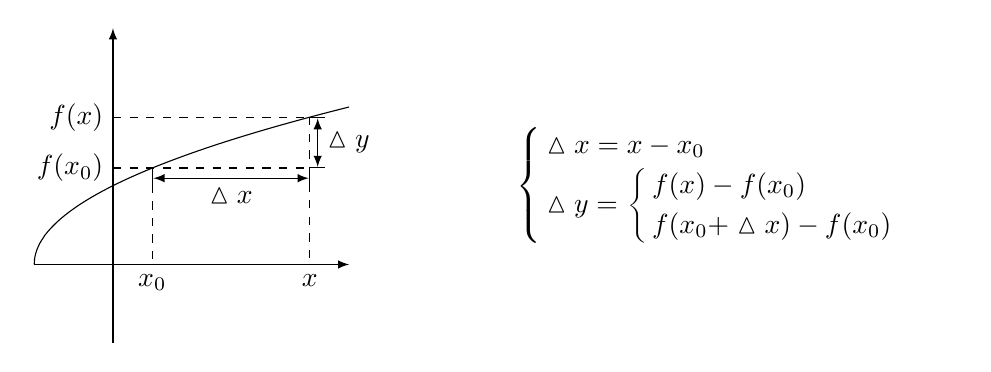
\begin{tikzpicture}[>=latex]
    \centering
    \begin{scope}
        \draw[->](0,0)--(4,0);
        \draw[->](1,-1)--(1,3);
        \draw[domain=0:4,samples=1000] plot(\x,{\x^(1/2)});
        \draw[dashed] (1.5,{1.5^(1/2)})--(1.5,0)node[below]{$x_0$};
        \draw[dashed] (3.5,{3.5^(1/2)})--(3.5,0)node[below]{$x$};
        \draw[dashed] (1,{1.5^(1/2)})node[left]{$f(x_0)$}--(2.5,{1.5^(1/2)})--(3.5,{1.5^(1/2)});
        \draw[|<->|] (1.5,{1.2^(1/2)})--(2.5,{1.2^(1/2)})node[below]{$\vartriangle x$}--(3.5,{1.2^(1/2)});
        \draw[dashed] (1,{3.5^(1/2)})node[left]{$f(x)$}--(3.5,{3.5^(1/2)});
        \draw[|<->|] (3.6,{3.5^(1/2)})--(3.6,{(3.5^(1/2)+1.5^(1/2))/2})node[right]{$\vartriangle y$}--(3.6,{1.5^(1/2)});
    \end{scope}
    \begin{scope}[xshift=6cm]
        \node at (0,1)[right]{$\begin{cases}
            \vartriangle x=x-x_0\\
            \vartriangle y=\begin{cases}
                f(x)-f(x_0)\\
                f(x_0+\vartriangle x)-f(x_0)
            \end{cases}
        \end{cases}$};
    \end{scope}
\end{tikzpicture}
$$Def2:\mbox{如果}\lim\limits_{\vartriangle x\to 0}\vartriangle y =\lim\limits_{\vartriangle x\to 0}\left[f(x_0+\vartriangle x)-f(x_0)\right]=0$$
$$\mbox{则称}f(x)\mbox{在}x_0\mbox{处连续}$$
\subsubsection{区间连续}
$\forall x_0\in\left[a,b\right]\begin{cases}
    \lim\limits_{x\to x_0}f(x)=f(x_0)&x_0\in\left(a,b\right) \Leftrightarrow f(x_0)=\begin{cases}
    \lim\limits_{x \to x_0^-}f(x)= f(x_0^-)\\
    \lim\limits_{x \to x_0^+}f(x)= f(x_0^+)
\end{cases}\\
    \lim\limits_{x\to x_0^+}f(x)=f(x_0^+)&x_0=a\ \left(\mbox{右连续}\right)\\
    \lim\limits_{x\to x_0^-}f(x)=f(x_0^-)&x_0=b\ \left(\mbox{左连续}\right)
\end{cases}$\\称在$\left[a,b\right]$内连续\\
有界:$\exists M>0,x\in\left[a,b\right]$时,$\left|f(x)\right|\geqslant M$\\
最大值:$\exists x_0\in\left[a,b\right]$时,$\forall x\in\left[a,b\right] ,f(x)\leqslant f(x_0)$称$f(x_0)$为$f(x)$在$\left[a,b\right]$上的最大值\\
最小值:$\exists x_0\in\left[a,b\right]$时,$\forall x\in\left[a,b\right] ,f(x)\geqslant f(x_0)$称$f(x_0)$为$f(x)$在$\left[a,b\right]$上的最小值\\
1,闭区间$\left[a,b\right]$上的连续函数$f(x)$有界,一定取得最大值与最小值。
\subsubsection{间断点}
1,$f(x)$无定义\\
2,$\lim\limits_{x\to x_0}f(x)$不存在\\
3.$\lim\limits_{x\to x_0}f(x)$存在,但$\lim\limits_{x\to x_0}f(x)\neq f(x_0)$\\
第一类间断点:$f(x_0^+)=\lim\limits_{x\to x_0^+}f(x)$与$f(x_0^-)=\lim\limits_{x\to x_0^-}f(x)$\\
第二类间断点:不是第一类的。
\subsection{连续函数的运算}
函数$f(x),g(x)$在$x=x_0$连续。
\begin{displaymath}
    \begin{split}
        \lim\limits_{x\to x_0}\left[f(x)\pm g(x)\right]&=\lim\limits_{x\to x_0}f(x)\pm \lim\limits_{x\to x_0}g(x)=f(x_0)\pm g(x_0)\\
        \lim\limits_{x\to x_0}\left[f(x)\cdot g(x)\right]&=\lim\limits_{x\to x_0}f(x)\cdot \lim\limits_{x\to x_0}g(x)=f(x_0)\cdot g(x_0)\\
        \lim\limits_{x\to x_0}\left[\frac{f(x)}{g(x)}\right]&=\frac{\lim\limits_{x\to x_0}f(x)}{\lim\limits_{x\to x_0}g(x)}=\frac{f(x_0)}{g(x_0)}\qquad \left(g(x_0)\neq 0\right)
    \end{split}
\end{displaymath}
反函数的连续性\\
若$y=f(x)$在区间$I_x$上单调增加,且连续。\\
则$y=f^-1(x)$在$I_y=\left\{y|y=f(x),x\in I_x\right\}$上也为单调增加,连续\\
$$\mbox{复合函数}\begin{cases}
    \mbox{内外都连续}\begin{cases}
    \lim\limits_{x\to x_0}g(x)=g(x_0)=u_0\\
    \lim\limits_{u\to u_0}f(x)=f(u_0)\\
    \lim\limits_{x\to x_0}f\left[g(x)\right]=f\left[g(x_0)\right]=f(\lim\limits_{x\to x_o}g(x))
\end{cases}\\
    \mbox{外连续}\begin{cases}
        x\rightarrow x_0\begin{cases}
        \lim\limits_{x\to x_0}g(x)=u_0\\
        \lim\limits_{u\to u_0}f(x)=f(u_0)\\
        \lim\limits_{x\to x_0}f\left[g(x)\right]=f(u_0)=f(\lim\limits_{x\to x_o}g(x))
    \end{cases}\\
        x\rightarrow \infty\begin{cases}
            \lim\limits_{x\to \infty}g(x)=u_0\\
            \lim\limits_{u\to u_0}f(x)=f(u_0)\\
            \lim\limits_{x\to \infty}f\left[g(x)\right]=f(u_0)=f(\lim\limits_{x\to \infty}g(x))
        \end{cases}
    \end{cases}
\end{cases}$$
\subsection{零点定理}
2,设$f(x)$在$\left[a,b\right]$上连续,且$f(a)\cdot f(b)<0$\\
则至少存在一点$\xi \in \left(a,b\right)$使$f(\xi)=0$
\subsection{介质定理}
设$f(x)$在$\left[a,b\right]$上连续,且$f(a)=A,f(b)=B$\\
$\forall C\in\left(A,B\right),$至少有一点$\xi,f(\xi)=C$

 %极限
\section{导数}\label{zhang_derivative}
\subsection{定义}
导数的概念从物理发展出来的。
$$v\left(t_0\right)=\lim\limits_{\vartriangle t\to 0}\frac{s\left(t_0+\vartriangle t\right)-s\left(t_0\right)}{\vartriangle t}$$
\begin{figure}[htp]
  \centering
  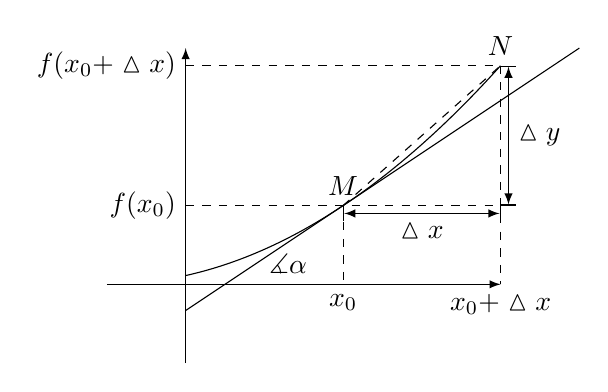
\begin{tikzpicture}[>=latex]
    \draw[->](0,0)--(5,0);
    \draw[->](1,-1)--(1,3);
    \draw[domain=1:5,samples=1000] plot(\x,{(\x^2)/9});
    \draw[domain=-2:3,samples=1000] plot(\x+3,{\x*(2/3)+1});
    \draw[dashed] (3,{(3^2)/9})--(3,0)node[below]{$x_0$};
    \draw[dashed] (3,{(3^2)/9})node[above]{$M$}--(5,{(5^2)/9})node[above]{$N$};
    \draw[dashed] (5,{(5^2)/9})--(5,0)node[below]{$x_0+\vartriangle x$};
    \node at (2.3,.5)[below]{$\measuredangle \alpha$};
    \draw[dashed] (1,{(3^2)/9})node[left]{$f(x_0)$}--(3,{(3^2)/9})--(5,{(3^2)/9});
    \draw[|<->|] (3,{(3^2)/9-.1})--(4,{(3^2)/9-.1})node[below]{$\vartriangle x$}--(5,{(3^2)/9-.1});
    \draw[dashed] (1,{(5^2)/9})node[left]{$f(x_0+\vartriangle x)$}--(5,{(5^2)/9});
    \draw[|<->|] (5.1,{(3^2)/9})--(5.1,{((5^2/9)+(3^2/9))/2})node[right]{$\vartriangle y$}--(5.1,{(5^2)/9});
\end{tikzpicture}
\end{figure}
$$NM\mbox{斜率}=\tan \beta=\frac{f\left(x_0+\vartriangle x\right)-f(x_0)}{\vartriangle x}=\frac{\vartriangle y}{\vartriangle x}$$
$$\mbox{斜率}k=\tan \alpha=\lim\limits_{\vartriangle x\to 0}\tan \beta=\lim\limits_{\vartriangle x\to 0}\frac{\vartriangle y}{\vartriangle x}=\frac{f\left(x_0+\vartriangle x\right)-f(x_0)}{\vartriangle x}$$
\subsubsection{导数定义}
$y=f(x)$在$x_0$的某邻域内有定义\\
给自变量的增量$\vartriangle x,\left(x_0+\vartriangle x\right)$仍在定义域内\\
函数得到了相应增量$\vartriangle y ,\vartriangle y =f\left(x_0+\vartriangle x\right)$\\
如果$\lim\limits_{\vartriangle x\to 0}\frac{f\left(x_0+\vartriangle x\right)-f(x_0)}{\vartriangle x}$存在,称$y=f(x)$在$x=x_0$处可导 \\
$\left(\mbox{极限值为}y=f(x)\mbox{在}x=x_0\mbox{处导数}\right)$
\begin{center}
  记$y'|_{x=x_0}=f'(x_0)=\lim\limits_{\vartriangle x\to 0}\frac{f(x_0+\vartriangle x)-f(x_0)}{\vartriangle x}$
  $$\lim\limits_{\vartriangle x\to 0}\frac{f(x_0+\vartriangle x)-f(x_0)}{\vartriangle x}\Leftrightarrow\lim\limits_{\vartriangle x\to x_0}\frac{f(x)-f(x_0)}{x-x_0}$$
\end{center}
\subsubsection{导函数定义}
$f(x)$在区间$I$内任意一点均可导。\\
$f'(x)=\lim\limits_{\vartriangle x\to 0}\frac{f(x_0+\vartriangle x)-f(x_0)}{\vartriangle x}$\\
称$f'(x)$为$y=f(x)$在区间$I$上的导函数
\subsubsection{闭区间可导定义}
$f(x)$在$[a,b]$可导$\Leftrightarrow\begin{cases}
  f'(x_0)  &x_0\in(a,b)\Leftrightarrow\begin{cases}
    \mbox{左导数}f_-'(x_0)=\lim\limits_{\vartriangle x\to 0^-}\frac{f(x_0+\vartriangle x)-f(x_0)}{\vartriangle x}\\
    \mbox{右导数}f_+'(x_0)=\lim\limits_{\vartriangle x\to 0^+}\frac{f(x_0+\vartriangle x)-f(x_0)}{\vartriangle x}
  \end{cases}\\
  f_+'(a) &x=a\\
  f_-'(a) &x=b
\end{cases}$
\subsubsection{导数与连续}
\begin{align}\label{derivative_continuity}
  f'(x)\mbox{存在}\Rightarrow f(x)\mbox{在}x=x_0\mbox{处连续}
\end{align}
\subsection{幂数,指数,对数}
\begin{align}
&\frac{d}{\mathrm{d}{x}}C = 0\label{derivative_1} \\
&\frac{d}{\mathrm{d}{x}}x^a = ax^{a-1} \label{derivative_2} \\
&\frac{d}{\mathrm{d}{x}}a^x = a^x\ln a \label{derivative_3}\\
&\frac{d}{\mathrm{d}{x}}e^x = e^x \label{derivative_4}\\
&\frac{d}{\mathrm{d}{x}}\log_a^x = \frac{1}{x\ln a} \label{derivative_5}\\
&\frac{d}{\mathrm{d}{x}} \ln{x} = \frac{1}{x} \label{derivative_6}
\end{align}

\subsection{三角函数}
\begin{align}
&\frac{d}{\mathrm{d}{x}}\sin x = \cos x \label{derivative_sin}\\
&\frac{d}{\mathrm{d}{x}}\arcsin x = \frac{1}{\sqrt{1-x^2}} \label{derivative_arcsin}\\
&\frac{d}{\mathrm{d}{x}}\csc x = -\csc x\cot x \label{derivative_csc}\\
&\frac{d}{\mathrm{d}{x}}\cos x = -\sin x \label{derivative_cos}\\
&\frac{d}{\mathrm{d}{x}}\arccos x = -\frac{1}{\sqrt{1-x^2}} \label{derivative_arccos}\\
&\frac{d}{\mathrm{d}{x}}\sec x = \sec x\tan x \label{derivative_sec}\\
&\frac{d}{\mathrm{d}{x}}\operatorname{arcsec}{x}=\frac{1}{\left|x\right|\sqrt{x^2-1}} \label{derivative_arcsec}\\
&\frac{d}{\mathrm{d}{x}}\tan x = \sec^2x \label{derivative_tan}\\
&\frac{d}{\mathrm{d}{x}}\arctan = \frac{1}{1+x^2} \label{derivative_arctan}\\
&\frac{d}{\mathrm{d}{x}}\cot x = -\csc^2x \label{derivative_cot}\\
&\frac{d}{\mathrm{d}{x}}\operatorname{arccot}{x} = -\frac{1}{1+x^2}\label{derivative_arccot}\\
&\frac{d}{\mathrm{d}{x}}\sinh x = \cosh x \label{derivative_sinh}\\
&\frac{d}{\mathrm{d}{x}}\cosh x = \sinh x \label{derivative_cosh}\\
&\frac{d}{\mathrm{d}{x}}\tanh x = \frac{1}{cosh^2 x}=1-\tanh^2x \label{derivative_tanh}\\
&\frac{d}{\mathrm{d}{x}}\operatorname{arcsinh}{x} =\frac{1}{\sqrt{x^2+1}} \label{derivative_arcsinh}\\
&\frac{d}{\mathrm{d}{x}}\operatorname{arccosh}{x} =\frac{1}{\sqrt{x^2-1}} \label{derivative_arccosh}\\
&\frac{d}{\mathrm{d}{x}}\operatorname{arctanh}{x} =\frac{1}{1-x^2} \label{derivative_arctanh}
\end{align}

\subsection{导数运算}
$$U=u(x),V=v(x),\mbox{均在}x\mbox{点可导},C\mbox{为常数}$$
\begin{align}
  \frac{d(CU)}{\mathrm{d}{x}}&= C\frac{d(U)}{\mathrm{d}{x}}\label{limit_operation_1}\\
  \frac{d(U+V)}{\mathrm{d}{x}}&=\frac{dU}{\mathrm{d}{x}}\pm \frac{dV}{\mathrm{d}{x}}\label{limit_operation_2}\\
  \frac{d(UV)}{\mathrm{d}{x}}&=\frac{dU}{\mathrm{d}{x}}V+\frac{dV}{\mathrm{d}{x}}U\label{limit_operation_3}\\
  \frac{d(\frac{U}{V})}{\mathrm{d}{x}}&=\frac{\frac{dU}{\mathrm{d}{x}}V-\frac{dV}{\mathrm{d}{x}}U}{V^2}\label{limit_operation_4}
\end{align}
\subsection{反函数求导}
如果函数$y=f(x)$在区间$(a,b)$内单调可导,且$f'(y)\neq 0$\\
$\begin{cases}
  \alpha=\min\{f(a)+0,f(b-0)\}\\
  \beta=\max\{f(a)+0,f(b-0)\}
\end{cases}$\\
则它的反函数$x=f^{-1}(y)$在区间$(\alpha,\beta)$内也可导
\begin{align}
  \left[f^{-1}(y)\right]'=\frac{1}{f'(x)} \label{derivative_of_inverse_function}
\end{align}
$$\frac{dy}{\mathrm{d}{x}}=\frac{1}{\frac{dx}{\mathrm{d}{y}}}$$
\subsection{复合函数求导}
\begin{center}
  设函数$\begin{cases}
    y=f(u)\mbox{在}U(u_0,\delta_0)\mbox{处有定义}\\
    u=g(x)\mbox{在}U(x_0,\eta_0)\mbox{处有定义}
  \end{cases}$\\
  $u_0=g(x_0),\mbox{且}f'(u)\mbox{和}g'(x)\mbox{都存在}$\\
  $\mbox{则复合函数}F(x)=f\left[g(x)\right]\mbox{在点}x_0\mbox{可导,且}$
  \begin{align}
    F'(x_0)=f'\left[g(x_0)\right]g'(x_0)\label{derivative_of_composite_functions}
  \end{align}
\end{center}
$$\frac{dy}{dx}=\frac{dy}{du}\cdot\frac{du}{dx}$$
\subsection{高阶求导}
$Def:\begin{cases}
  \mbox{一阶导数} &y'\Leftrightarrow \frac{dy}{dx}\\
  \mbox{二阶导数}&y''\Leftrightarrow \frac{d^2y}{dx^2}\\
  \mbox{三阶导数}&y'''\Leftrightarrow \frac{d^3y}{dx^3}\\
  \mbox{三阶以上n阶导数}&y^{(n)}\Leftrightarrow \frac{d^ny}{dx^n}\\
\end{cases}$
\subsection{高阶求导公式}
\begin{align}
  \frac{d^n}{dx}e^x&=e^x\\
  \frac{d^n}{dx}a^x&=a^x\left(ln a\right)^n\\
  \frac{d^n}{dx}x^\mu&=A_\mu^nx^{\mu-n}\\
  \frac{d^n}{dx}\left(\frac{1}{x+a}\right)&=\frac{(-1)^nn!}{(x+a)^{n+1}}\\
  \frac{d^n}{dx}\ln(x+a)&=\frac{(-1)^{n-1}(n-1)!}{(x+a)^n}\\
  \frac{d^n}{dx}\sin x&=\sin(x+n\frac{\pi}{2})\\
  \frac{d^n}{dx}\cos x&=\cos(x+n\frac{\pi}{2})\\
  \frac{d^n}{dx}\left[f(ax+b)\right]&=a^n\cdot\frac{d^nf(ax+b)}{d(ax+n)}
\end{align}
\subsection{高阶求导运算法则}
\begin{align}
  \frac{d^n}{dx}(u\pm v)&=\frac{d^nu}{dx}\pm\frac{d^nv}{dx}\\
  \mbox{莱布紫泥公式}\qquad(uv)^{n}&=\sum_{k=0}^{n}C_{n}^{k}u^{(n-k)}\cdot v^k
\end{align}
\subsection{隐函数求导}
\subsection{参数方程求导} %导数
\section{微分}\label{zhang_differential}
%\begin{figure}[htp]
%    \centering
 %   \begin{tikzpicture}[>=latex]
      %\draw[-](0,0)--(3,0)--(3,3)--(0,3)--(0,0);
      %\draw[-](2,0)--(2,3);
    %  \draw[-](0,2)--(3,2);
   %   \node at(1,1){$A=x_0^2$};
  %\end{tikzpicture}
 % \end{figure}
  \subsection{定义}
  \begin{center}
    设函数$f(x)$在点$x_0$的一个邻域内有定义。$\vartriangle y=f(x_0+\vartriangle x)-f(x_0)$\\\
    如果$\vartriangle y$可以表示为$\vartriangle y=A\vartriangle x+\circ (\vartriangle x)$其中$A$为与$\vartriangle x$无关的常数\\
    则称$f(x)$在点$x_0$可微,$A\vartriangle x$称为$f(x)$在点$x_0$处的微分。\\
    $\mbox{记作:}dy=A\vartriangle x$
  \end{center}
\begin{figure}[htp]
   \centering
    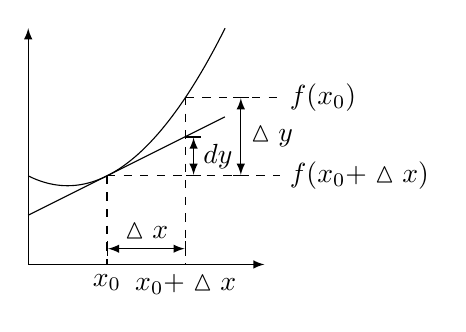
\begin{tikzpicture}[>=latex]
      \draw[->](0,0)--(3,0);
      \draw[->](0,0)--(0,3);
      \draw[domain=0:2.5,samples=1000] plot(\x,{((\x-.5)^2)*(1/2)+1});
      \draw[domain=0:2.5,samples=500] plot(\x,{(\x-1)*(1/2)+9/8});
      \draw[|<->|] (2.1,{(2-1)*(1/2)+9/8})--(2.1,{(((1-.5)^2)*(1/2)+1+(2-1)*(1/2)+9/8)/2})node[right]{$dy$}--(2.1,{((1-.5)^2)*(1/2)+1});
      \draw[dashed](1,{((1-.5)^2)*(1/2)+1})--(1,0)node[below]{$x_0$};
      \draw[dashed](2,{((2-.5)^2)*(1/2)+1})--(2,0)node[below]{$x_0+\vartriangle x$};
     % \node at (3,-1)[below]{常函数\ $f(x)=a\{a\in R\}$};
      \draw[|<->|] (1,.2)--(1.5,.2)node[above]{$\vartriangle x$}--(2,.2);
      \draw[dashed](2,{((2-.5)^2)*(1/2)+1})--(3.2,{((2-.5)^2)*(1/2)+1})node[right]{$f(x_0)$};
      \draw[dashed](1,{((1-.5)^2)*(1/2)+1})--(3.2,{((1-.5)^2)*(1/2)+1})node[right]{$f(x_0+\vartriangle x)$};
      \draw[|<->|](2.7,{((2-.5)^2)*(1/2)+1})--(2.7,{(((2-.5)^2)*(1/2)+1+((1-.5)^2)*(1/2)+1)/2})node[right]{$\vartriangle y$}--(2.7,{((1-.5)^2)*(1/2)+1});
    \end{tikzpicture}
\end{figure}
\begin{align}
    \mbox{可微}\Rightarrow\mbox{可导}\label{differential_to_derivative}\\
    \mbox{可导}\Rightarrow\mbox{可微}\label{derivative_to_differential}
\end{align}

\subsection{微分法则}
\subsubsection{核心根本}
\begin{figure}[htp]
    \centering
    \begin{tikzpicture}[>=latex]
      \draw[->](1.5,.2)--(1.5,.5)--(3,.5)--(3,.2);
      \node at(2.25,.5)[above]{积分};
      \draw[<-](1.5,-.2)--(1.5,-.5)--(3,-.5)--(3,-.2);
      \node at(2.25,-.5)[below]{求导};
      \node at(.5,0){$dy=$};
      \node at(1.5,0){$f'(x)$};
      \node at(2.3,0){$d$};
      \node at(3,0){$x$};
  \end{tikzpicture}
\end{figure}
\subsubsection{四则运算}
\begin{align}
    d\left(u\pm v\right)=du\pm dv\label{differential_operation_rule_1}\\
    d(uv)=vdu+udv \label{differential_operation_rule_2}\\
    d\left(\frac{u}{v}\right)=\frac{vdu+udv}{v^2} \label{differential_operation_rule_3}
\end{align}
\subsubsection{复合运算}
\begin{center}
    可微$\begin{cases}
        y=f(u)\\
        u=g(x)
    \end{cases}\Rightarrow \begin{cases}
        dy=f'(u)du\\
        du=g'(x)dx
    \end{cases}$则$y=f(g(x))$也可微\\
    且$  dy=f'(u)du=f'(u)g(x)dx$\\
    $u$是否为中间变量都成立,微分的不变性。
\end{center}
\subsubsection{近似计算公式}
\begin{center}
    $\vartriangle x\rightarrow 0, dy\approx \vartriangle y\begin{cases}
        dy=f'(x_0)\vartriangle x\\
        \vartriangle y=f(x_0+\vartriangle x)-f(x_0)
    \end{cases}\begin{cases}
        f(x_0+\vartriangle x)\approx f(x_0)+f'(x_0)\vartriangle x\\
        f(x)\approx f(x_0)+f'(x_0)(x-x_0)\\
        x_0=0\begin{cases}
            f(x)\approx f(0)+f'(0)x\\
            \sqrt{n}\approx 1+\frac{1}{n}x\\
            \sin x \approx x\\
            \tan x \approx x\\
            e^x \approx 1+x\\
            \ln(1+n)\approx x
        \end{cases}
    \end{cases}$\\
\end{center}
\subsubsection{奇偶函数导数}
\begin{center}
    偶函数导数为奇函数$f(x)=f(-x)\Leftrightarrow f'(x)=-f'(-x)$\\
    奇函数导数为偶函数$f(x)=-f(-x)\Leftrightarrow f'(x)=f'(-x)$
\end{center}
\subsubsection{区间恒为0}
$$\mbox{若}f'(x)\mbox{在区间恒为零,则}f(x)\mbox{在区间}I\mbox{上为一常数}$$
$\mbox{设}x_1,x_2\mbox{为区间}I\mbox{内任意两点}x_1<x_2$\\
$f(x_2)-f(x_1)=f'(\xi)(x_2-x_1)\equiv 0 $\\
$f(x_2)\equiv f(x_1)=C$
\subsection{中值定理}
\subsubsection{费马引理}
\begin{center}
    $f(x)\qquad \forall x\in \mathring{U}(x_0)\begin{cases}
        f(x)\leqslant f(x_0)\qquad f(x)\mbox{在}x_0\mbox{处取极大值}\\
        f(x)\geqslant f(x_0)\qquad f(x)\mbox{在}x_0\mbox{处取极小值}
    \end{cases}$
\end{center}
\begin{equation}
    \mbox{如果可导函数}y=f(x)\mbox{在}x_0\mbox{取极值,则}f'(x_0)=0\label{Fermat_Lemma}
\end{equation}
\subsubsection{罗尔定理}
\begin{center}
    $\mbox{如果函数}f(x)\mbox{满}\begin{cases}
    \mbox{在闭区间$\left[a,b\right]$上连续}\\
    \mbox{在开区间(a,b)可导}\\
    f(a)=f(b)
    \end{cases}$\\
    \begin{align}
        \mbox{则至少有一点}\xi\in(a,b),f'(\xi)=0\label{Rolle's theorem}
    \end{align}
\end{center}
\begin{figure}[htp]
    \centering
    \begin{tikzpicture}[>=latex]
        \draw[->](-.5,0)--(8,0)node[right]{$x$};
        \draw[->](0,-.5)--(0,4)node[above]{$y$};
        \draw[domain=0:2*pi,samples=1000] plot(\x+1,{sin(\x r)+2});      
        \draw[dashed] (1,{2})--(1,0)node[below]{$a$};    
        \draw[dashed] ({1+(2*pi)},{2})--({1+(2*pi)},0)node[below]{$b$};   
        \draw[dashed] (1,{2})node[left]{$A$}--({1+(2*pi)},{2})node[right]{$B$};
        \draw[dashed] ({1+(.5*pi)},{sin(pi/2 r)+2})--({1+(.5*pi)},0)node[below]{$\xi$};
        \draw[dashed] (1.5,{sin(pi/2 r)+2})--({.5+pi},{sin(pi/2 r)+2});
    \end{tikzpicture}
\end{figure}
\subsubsection{拉格朗日定理$\left(\mbox{微分中值定理}\right)$}
\begin{figure}[htp]
    \centering
    \begin{tikzpicture}[>=latex]
        \draw[->](-.5,0)--(8,0)node[right]{$x$};
        \draw[->](0,-.5)--(0,4)node[above]{$y$};
        \draw[domain=0:2*pi,samples=1000] plot(\x+1,{sin(\x r)+(\x/2)+1});
        \draw[dashed](1,1)--(1,0)node[below]{$a$};
        \draw[dashed]({1+(2*pi)},{(2*pi/2)+1})--({1+(2*pi)},0)node[below]{$b$};
        \draw[dashed](1,1)--({1+(2*pi)},{(2*pi/2)+1});
        \draw[dashed]({1+(pi/2)},{sin(pi/2 r)+(pi/4)+1})--({1+(pi/2)},0)node[below]{$\xi$};
        \draw[dashed]({1+(pi/2)-1},{sin(pi/2 r)+(pi/4)+1-.5})--({1+(pi/2)+1},{sin(pi/2 r)+(pi/4)+1+.5});
    \end{tikzpicture}
\end{figure}
\begin{center}
    $\mbox{如果函数}f(x)\mbox{满}\begin{cases}
    \mbox{在闭区间$\left[a,b\right]$上连续}\\
    \mbox{在开区间(a,b)可导}
    \end{cases}$\\
    $\mbox{则至少有一点}\xi\in(a,b)$\\
    \begin{align}
        f'(\xi)=\frac{f(b)-f(a)}{b-a}\Leftrightarrow f(b)-f(a)=f'(x)(b-a)\label{Lagrange's theorem}
    \end{align}
    在区间$\left[x,x+\vartriangle x\right]$用拉格朗日定理。\\
    $f(x+\vartriangle x)-f(x)=f'(\xi)\vartriangle x$\\
    $\xi\in(x,x+\vartriangle x)$记作:\ $\xi=x+\theta \vartriangle x\qquad 0<\theta <1$\\
    $f(x+\vartriangle x)-f(x)=f(x+\theta \vartriangle x)\vartriangle x$\\
    $\vartriangle y=f(x+\theta \vartriangle x)\vartriangle x$\\

\end{center}
\subsubsection{柯西定理}
 %微分
\section{不定积分}
\subsection{概念}
\subsubsection{原函数}
$$\forall x\in I,\ F'(x)=f(x),\quad F(x)\mbox{为}f(x)\mbox{的一个原函数}$$
\begin{align}
    \mbox{函数}f(x)\mbox{在区间}I\mbox{上连续一定有}F(x),\mbox{使}F'(x)=f(x)
\end{align}
\subsubsection{不定积分}
区间$I$上,$f(x)$带有任意常数的原函数,称为$f(x)$在区间I上的不定积分。\\
记作:
$$\int f(x)dx\quad\begin{cases}
    \int&\mbox{积分符号}\\
    f(x)&\mbox{被积函数}\\
    f(x)dx\ &\mbox{被积表达式}\\
    x &\mbox{积分变量}
\end{cases}$$
$\mbox{如果}F(x)\mbox{是}f(x)\mbox{的一个原函数}$
$$\int f(x)dx=F(x)+C$$
\subsubsection{不定积分性质}
$$\left[\int f(x)dx\right]'=f(x)$$
\subsection{幂数,指数,对数}
\begin{align}
&\int k dx=kx +C\\
&\int x^a \mathrm{d}{x} = \frac{x^{a+1}}{a+1} + C\\
&\int a^x \mathrm{d}{x} = \frac{a^x}{\ln a} + C\\
&\int e^x \mathrm{d}{x} = e^x + C\\
&\int \frac{1}{x} \mathrm{d}{x} = \ln\left|x\right| + C
\end{align}
\subsection{三角函数}
\begin{align}
&\int \frac{1}{1+x^2}=\arctan x + C\\
&\int\sin x \mathrm{d}{x} = -\cos x + C\\
&\int\frac{1}{\sqrt{1-x^2}}\mathrm{d}{x} =\begin{cases}
    \arcsin x + C\\
    -\arccos x +C_1
\end{cases}  \\
&\int\csc x\cot x \mathrm{d}{x} = -\csc x + C\\
&\int\cos x \mathrm{d}{x} = \sin x + C \\
&\int\sec x \tan x\mathrm{d}{x} = \sec x + C \\
&\int\sec^2 x\mathrm{d}{x} = \tan x + C \\
&\int\csc^2 x\mathrm{d}{x} = -\cot x +C \\
&\int\frac{1}{\left|x\right|\sqrt{x^2-1}}\mathrm{d}{x} = \operatorname{arcsec} x + C \\
&\int\frac{1}{1+x^2}\mathrm{d}{x} = \tan x + C\\
&\int\sinh x \mathrm{d}{x} = \cosh x + C\\
&\int\cosh x \mathrm{d}{x} = \sinh x + C
\end{align}
\subsection{积分运算}
 %积分
\section{零散的一些}
\begin{align}
\sum\limits_{k=0}^{n}q^k = \frac{1-q^{n+1}}{1-q}
\end{align}
\noindent\rule{\textwidth}{0.4pt}
$$A_N = \sum\limits_{k = 0}^{n}q^k \qquad qA_N = \sum\limits_{k = 1}^{n+1}q^k$$
$$A_N - qA_N = \sum\limits_{k = 0}^{n}q^k -\sum\limits_{k=1}^{n+1}q^k = 1-q^{n+1}$$
$$A_N = \frac{1-q^{n+1}}{1-q}$$
\noindent\rule{\textwidth}{0.4pt}

\begin{align}
&\log_{10}{x} = \lg_{x} \\
&\log_{e}{x} = \ln_{x}\\
&\log_{b}{xy} = \log_{b}{x} + \log_{b}{y}\\
&\log_{\left(b^n\right)}{x} = \frac{1}{n}\log_{b}{x} \\
&\log_{b}{x^n} = n\log_{b}{x} \\
&\log_{b}{x} = \frac{\log_{c}{x}}{\log_{c}{b}}
\end{align}
\noindent\rule{\textwidth}{0.4pt}
$$b^n = x\qquad b^m =y$$
$$b^{n+m} = xy$$
$$\log_{b}{xy} = n + m = \log_{b}{x} + \log_{b}{y}$$
% 长横线
\noindent\rule{\textwidth}{0.4pt}
$$b^n = x$$
$$\log_{b}{x} = n$$
$$\frac{1}{n}\log_{b}{x}= 1 = \log_{\left(b^n\right)}{x}$$
% 带有一定垂直空间的长横线
\noindent\rule[\fill]{\textwidth}{0.4pt}
$$b^1 = x^n \qquad b^{\frac{1}{n}} = x$$
$$n\log_{b}{x} = 1 = \log_{b}{x^n}$$
\noindent\rule[\fill]{\textwidth}{0.4pt}
$$\log_{b}{x} = log_{c^{\left(\log_{c}{b}\right)}}{c^{\left(\log_{c}{x}\right)}}=\frac{\log_{c}{x}}{\log_{c}{b}}$$
\noindent\rule[\fill]{\textwidth}{0.4pt}
$$\left(a+b\right)^n=\sum_{m = 0}^{n} C_n^m a^{n-m}b^m $$
\noindent\rule[\fill]{\textwidth}{0.4pt}
$$a^2-b^2=\left(a-b\right)\left(1+b\right)$$
$$a^3-b^3=\left(a-b\right)\left(a^2+ab+b^2\right)$$
$$a^n-b^n=\left(a-b\right)\sum_{m=0}^{n-1}\left(a^{n-m}b^{m}\right)=\left(a-b\right)\left(a^{n-1}+a^{n-2}b+\cdots+ab^{n-2}+b^{n-1}\right)$$ %零散的
\section{证明}
\subsection{\centering 第\ref{zhang_trigonometric_function}章}
\textbf{\large \ref{eq:hyperbolic_functions_1}}
\begin{displaymath}
\begin{split}
\sinh x\cosh x &= \left(\frac{e^x-e^{-x}}{2}\right)\left(\frac{e^x+e^{-x}}{2}\right) \\
&=\left(\frac{1}{2}\right)\left(\frac{e^{2x}-e^{-2x}}{2}\right) \\
&= \frac{1}{2}\sinh (2x) \\
\sinh (2x) &= 2\sinh x\cosh x
\end{split}
\end{displaymath}

\textbf{\large \ref{eq:hyperbolic_functions_2}}
\begin{displaymath}
\begin{split}
\cosh^2x-\sinh^2x &=\left(\frac{e^x+e^{-x}}{2}+\frac{e^x-e^{-x}}{2}\right)\left(\frac{e^x+e^{-x}}{2}-\frac{e^x-e^{-x}}{2}\right) \\
&= e^x\times e^{-x} \\
&=1
\end{split}
\end{displaymath}

\textbf{\large \ref{eq:hyperbolic_functions_3}}
\begin{displaymath}
\begin{split}
\cosh^2x+\sinh^2x &=\left(\frac{e^x+e^{-x}}{2}\right)^2+\left(\frac{e^x-e^{-x}}{2}\right)^2 \\
&=\frac{2e^{2x}+2e^{-2x}}{4} \\
&=\frac{e^{2x}+e^{-2x}}{2} \\
&=\cosh (2x)
\end{split}
\end{displaymath}

\textbf{\large \ref{eq:hyperbolic_functions_4}}
\begin{displaymath}
\begin{split}
\cosh (2x)  &=\cosh^2x+\sinh^2x \\
&=\sinh^2x +1 +\sinh^2x \\
&=2\sinh^2x +1 \\
\cosh x &=2\sinh^2\frac{x}{2}+1
\end{split}
\end{displaymath}

\subsection{\centering 第\ref{zhang_function}章}
\textbf{\large \ref{monotonous_1}}
\begin{displaymath}
    \begin{split}
        \mbox{设}\forall \ x_1,x_2&\in\left[a,b\right],x_1<x_2\\
        f(x_2)-f(x_1)&=f'(\xi)(x_2-x_1)\qquad \xi\in(x_1,x_2)\subset[a,b]\\
        f'(\xi)>0 ,&\ (x_2-x_1)>0\\
        f(x_2)-f(x_1)&>0\\
        f(x_2)&>f(x_1)
    \end{split}
\end{displaymath}
\textbf{\large \ref{monotonous_2}}
\begin{displaymath}
    \begin{split}
        \mbox{设}\forall\ x_1,x_2&\in\left[a,b\right],x_1<x_2\\
        f(x_2)-f(x_1)&=f'(\xi)(x_2-x_1)\qquad \xi\in(x_1,x_2)\subset[a,b]\\
        f'(\xi)<0 ,&\ (x_2-x_1)>0\\
        f(x_2)-f(x_1)&<0\\
        f(x_2)&<f(x_1)
    \end{split}
\end{displaymath}

\textbf{\large \ref{monotonous_3}}
\begin{center}
    $\mbox{设}\forall\  x_1,x_2\in\left[a,b\right],x_1<x_2,x_0=\frac{x_1+x_2}{2},x_0-x_1=x_2-x_0=h$\\
        $\varphi= \ding{173}f(x_0)-f(x_1)=f'(\xi_1)(x_0-x_1)\qquad \xi_1\in(x_1,x_0)$\\
        $\psi =f(x_2)-f(x_0)=f'(\xi_2)(x_2-x_0)\qquad \xi_2\in(x_0,x_2)$
\end{center}
\begin{displaymath}
    \begin{split}
        \psi-\varphi=f(x_2)+f(x_1)-2f(x_0)&=\left[f'(\xi_2)-f'(\xi_1)\right]h\\
         &=f''(\xi)(\xi_2-\xi_1)h\\
         \mbox{因为}\ f''(x)>0,f''(\xi)>0,h&=x_0-x_1>0\\
         f(x_2)+f(x_1)-2f(x_0)&>0\\
        f(x_2)+f(x_1)&>2f(x_0)\\
        f(x_0)&<\frac{f(x_2)+f(x_1)}{2}\\
        f(\frac{x_1+x_2}{2})&<\frac{f(x_2)+f(x_1)}{2}
    \end{split}
\end{displaymath}

\textbf{\large \ref{Arc_differentiation}}
$$\vartriangle s=\wideparen{M_0M'}-\wideparen{M_0M}=\wideparen{MM'},\quad \left|MM'\right|^2=(\vartriangle x)^2+(\vartriangle y)^2,\quad \lim\limits_{M'\to M}\frac{\left|\wideparen{MM'}\right|}{\left|MM'\right|}=1$$
\begin{align*}
    \left(\frac{\vartriangle s}{\vartriangle x}\right)^2=\left|\frac{\wideparen{MM'}}{\vartriangle x}\right|^2
   &=\left(\frac{\wideparen{MM'}}{\left|MM'\right|}\right)^2\cdot\left(\frac{\left|MM'\right|}{\vartriangle x}\right)^2\\
   &=\left(\frac{\wideparen{MM'}}{\left|MM'\right|}\right)^2\cdot\frac{(\vartriangle x)^2+(\vartriangle y)^2}{(\vartriangle x)^2}\\
   &=\left(\frac{\wideparen{MM'}}{\left|MM'\right|}\right)^2\cdot\left[1+\left(\frac{\vartriangle y}{\vartriangle x}\right)^2\right]\\
   \lim\limits_{\vartriangle x \to 0}\left(\frac{\vartriangle s}{\vartriangle x}\right)^2&= \lim\limits_{\vartriangle x \to 0}\left(\frac{\wideparen{MM'}}{\left|MM'\right|}\right)^2\cdot\lim\limits_{\vartriangle x \to 0}\left[1+\left(\frac{\vartriangle y}{\vartriangle x}\right)^2\right]\\
   (\vartriangle x \rightarrow 0,\vartriangle M' \rightarrow M)\qquad  &= \lim\limits_{M' \to M}\left(\frac{\wideparen{MM'}}{\left|MM'\right|}\right)^2\cdot\lim\limits_{\vartriangle x \to 0}\left[1+\left(\frac{\vartriangle y}{\vartriangle x}\right)^2\right]\\
    \left(\frac{ds}{dx}\right)^2&=1\cdot (1+(y')^2)\\
    \frac{ds}{dx}&=\sqrt{1+(y')^2}=\sqrt{1+\left[f'(x)\right]^2}\\
    ds&=\sqrt{1+\left[f'(x)\right]^2}dx=\sqrt{(dx)^2+(dy)^2}
\end{align*}

\textbf{\large \ref{Mean_curvature}}
\begin{align*}
    \left|\frac{d\alpha}{ds}\right|&=\left|\frac{d\alpha}{dx}\cdot\frac{dx}{ds}\right|\\
    &=\left|\frac{d\arctan y'}{dx}\cdot\frac{1}{\sqrt{1+(y')^2}}\right|\\
    &=\left|\frac{y''}{1+(y')^2}\cdot\frac{1}{\sqrt{1+(y')^2}}\right|\\
    &=\frac{\left|y''\right|}{\left(1+(y')^2\right)^{\frac{3}{2}}}
\end{align*}

\textbf{\large \ref{Point_curvature}}
\begin{align*}
    \frac{dy}{dx}&=\frac{\psi'(t)}{\phi'(t)}\\
    \frac{d^2y}{dx^2}&=\frac{d\frac{\psi'(t)}{\phi'(t)}}{dt}\cdot\frac{dt}{dx}
=\frac{\psi''(t)\phi'(t)-\psi'(t)\phi''(t)}{\left[\phi'(t)\right]^2}\cdot\frac{1}{\phi'(t)}\\
&=\frac{\psi''(t)\phi'(t)-\psi'(t)\phi''(t)}{\left[\phi'(t)\right]^3}\\
    \left|\frac{d\alpha}{ds}\right|&=\frac{\left|y''\right|}{\left(1+(y')^2\right)^{\frac{3}{2}}}\\
    &=\frac{\psi''(t)\phi'(t)-\psi'(t)\phi''(t)}{\left[\phi'(t)\right]^3}\cdot\frac{1}{\left\{1+\left[\frac{\psi'(t)}{\phi'(t)}\right]^2\right\}^{\frac{3}{2}}}\\
    &=\frac{\psi''(t)\phi'(t)-\psi'(t)\phi''(t)}{\left\{\left|\psi'(t)\right|^2+\left[\phi'(t)\right]^2\right\}^{\frac{3}{2}}}
\end{align*}

\subsection{\centering 第\ref{zhang_limit}章}
\textbf{\large \ref{limit_sequence}}
\begin{displaymath}
    \begin{split}
        \mbox{反设}&\lim\limits_{n \to \infty}x_n =a,\ \lim\limits_{n \to \infty}x_n =b,\mbox{且}a<b\\
        \varepsilon&=\frac{b-a}{3}\begin{cases}
            \exists N_1,\ n>N_1,\ \left|x_n-a\right|<\frac{b-a}{3}\\
            \exists N_2,\ n>N_2,\ \left|x_n-b\right|<\frac{b-a}{3}
        \end{cases}\\
        N&=\max\{N_1,N_2\},\ n>N\Rightarrow\begin{cases}
            n>N_1\\
            n>N_2
        \end{cases}\\
        b-a&=\left|(x_n-a)-(x_n-b)\right|\\
        &\leqslant \left|x_n-a\right|+\left|x_n-b\right|\\
        &<\frac{b-a}{3}+\frac{b-a}{3}\\
        &<\frac{2(b-a)}{3}
    \end{split}
\end{displaymath}

\textbf{\large \ref{sequence_bounded_1}}
    \begin{center}
       $\varepsilon =1,\ \exists N>0,\ \mbox{当n>N时}\left|X_n-a\right|<1$\\
        $\left|X_n\right|=\left|(X_n-a)+a\right|$\\
        $\qquad\leqslant \left|x_n-a\right|+\left|a\right|$\\
        $\leqslant 1+\left|a\right|$\\
        $M=\max\{\left|X_n\right|,\left|X_2\right|,\dots,\left|X_n\right|,1+\left|a\right|\}$\\
        $\forall n,\ \left|X_n\right|\leqslant M$
    \end{center}
\textbf{\large \ref{Serial_number_preservation_a}}
    \begin{center}1\end{center}
    $\mbox{由于}\lim\limits_{n\to\infty}x_n = a,\mbox{且}a>0$\\
    $\varepsilon = \frac{a}{2},\ \exists N>0,n>N$\\
    $\left|x_n-a\right|<\varepsilon$\\
    $\left|x_n-a\right|<\frac{a}{2}$\\
    $-\frac{a}{2}<x_n-a<\frac{a}{2}$\\
    $\frac{a}{2}<x_n<1$
    \begin{center}2\end{center}
    用反证法,反设$a<0$.从某项起$x_n<0$矛盾

\textbf{\large \ref{Serial_number_preservation_b}}
\begin{displaymath}
    \begin{split}
        x_n&=b_n-a_n\\
        \lim\limits_{n\to\infty} x_n &= \lim\limits_{n\to\infty} b_n-\lim\limits_{n\to\infty}a_n\\
        \lim\limits_{n\to\infty} x_n &=b-a>0\\
        \lim\limits_{n\to\infty} x_n &>0 \\
        b_n-a_n&=x_n > 0\\
        b_n&>a_n
    \end{split}
\end{displaymath}

\textbf{\large \ref{limit_left_right}}
$\lim\limits_{x\to x_0}f(x)\mbox{存在}\Rightarrow \lim\limits_{x\to x_0^+}f(x)=\lim\limits_{x\to x_0^-}f(x)$
\begin{center}
    设$\lim\limits_{x\to x_0}=A$\\
    $0<\left|x-x_0\right|<\delta,\ \left|f(x)-A\right|<\varepsilon$\\
    $0<\left|x-x_0\right|<\delta\Leftrightarrow x\in \mathring{U}(x_0,\delta)$
    $\begin{cases}
        \mbox{当}x_0<x<x_0+\delta\mbox{时}0<\left|x-x_0\right|<\delta,\ \left|f(x)-A\right|<\varepsilon,\ \lim\limits_{x\to x_0^+}f(x)=A\\
        \mbox{当}x_0-\delta<x<x_0\mbox{时}0<\left|x-x_0\right|<\delta,\ \left|f(x)-A\right|<\varepsilon,\ \lim\limits_{x\to x_0^-}f(x)=A
    \end{cases}$
    $\lim\limits_{x\to x_0^+}f(x)=A =\lim\limits_{x\to x_0^-}f(x)$
\end{center}
$\lim\limits_{x\to x_0}f(x)\mbox{存在}\Leftarrow\lim\limits_{x\to x_0^+}f(x)=\lim\limits_{x\to x_0^-}f(x)$
\begin{center}
    $A=\begin{cases}
    \lim\limits_{x\to x_o^+},\forall\varepsilon>0,\exists\delta_1>0,x_0<x<x_0+\delta_1,\left|f(x)-A\right|<\varepsilon\\
    \lim\limits_{x\to x_o^-},\forall\varepsilon>0,\exists\delta_2>0,x_0-\delta_2<x<x_0,\left|f(x)-A\right|<\varepsilon\\
    \end{cases}$\\
    $\delta = \min\{\delta_1,\delta_2\}$\\
    $0<\left|x-x_0\right|<\delta\begin{cases}
        x>x_0,x_0<x<x_0+\delta\leqslant x_0+\delta_1,\  \left|f(x)-A\right|<\varepsilon\\
        x<x_0,x_0-\delta_2\leqslant x_0+\delta<x<x_0,\ \left|f(x)-A\right|<\varepsilon
    \end{cases}$\\
    $\lim\limits_{x\to x_0}f(x)=A$
\end{center}

\textbf{\large \ref{limit_infinitesimal}}
\begin{center}
   $\lim\limits_{x\to x_o}f(x)=A\Rightarrow \begin{cases}
    \alpha\mbox{为}x\rightarrow x_0 \mbox{时的无穷小}\\
    f(x)=\alpha+A
\end{cases}$\\
设$\lim\limits_{x\to x_o}f(x)=A,\ \mbox{记}f(x)-A=\alpha$\\
只需证$\alpha$为无穷小。\\
$\forall\varepsilon>0,\exists\delta>0,\mbox{当}0<\left|x-x_0\right|<\delta,\mbox{时}\left|f(x)-A\right|<\varepsilon$\\
即$\left|\alpha-0\right|<\varepsilon$\\
$\alpha\mbox{为}x\rightarrow x_0\mbox{时的无穷小}$\\
$\lim\limits_{x\to x_o}f(x)=A\Leftarrow \begin{cases}
    \alpha\mbox{为}x\rightarrow x_0 \mbox{时的无穷小}\\
    f(x)=\alpha+A
\end{cases}$\\
$\forall \varepsilon >0,\ \exists \delta >0,\ \mbox{当}0<\left|x-x+0\right|<\delta,\ \left|\alpha\right|<\varepsilon$\\
$\mbox{即}\left|f(x)-A\right|<\varepsilon$
$\lim\limits_{x\to x_0}f(x)=A$
\end{center}


\textbf{\large \ref{Infinity_infinitesimal}}
\begin{center}
    设$\lim\limits_{x\to x_0}f(x)=\infty$\\
对$f(x)$为$x\rightarrow$时无穷大\\
对于$M=\frac{1}{\varepsilon}$.存在$\delta>0$\\
当$0<\left|x-x_0\right|<\delta$时\\
$\left|f(x)\right|>M=\frac{1}{\varepsilon}$\\
$\left|\frac{1}{f(x)}\right|<\varepsilon$\\
$\frac{1}{f(x)}$为$x\rightarrow x_0$时的无穷小
\end{center}

\textbf{\large \ref{Extreme Four Operations_2}}
\begin{displaymath}
    \begin{split}
        f(x)g(x)&=\left[A+\alpha\right]\left[B+\beta\right]\\
        &=AB+A\beta+B\alpha+\beta\alpha\\
        &=AB+\gamma\qquad\qquad(\gamma\mbox{为无穷小})\\
        \lim\left[f(x)g(x)\right]&=AB+\gamma=\lim f(x)\lim g(x)
    \end{split}
\end{displaymath}

\textbf{\large \ref{eq:squeeze_theorem}}
\begin{center}
    $\forall \varepsilon > 0$\\
$\left|x_n-a\right|<\varepsilon\qquad\forall n>N_1$\\
$\left|y_n-a\right|<\varepsilon\qquad\forall n>N_2$\\
$\mbox{令}N = \max\left\{{N_1,N_2,N_0}\right\}\mbox{,则当}n > N\mbox{时有}$\\
$a-\varepsilon<x_n\le z_n\le y_n < a+\varepsilon$\\
$\left|z_n-a\right|<\varepsilon$\\
$\lim\limits_{{n}\to{\infty}}z_n = a$
\end{center}

\textbf{\large \ref{limit_3_1}}
\begin{displaymath}
    \begin{split}
        \left|f(x)-\sin x_0\right|&=\left|\sin x-\sin x_0\right|\\
                                &=\left|2\cos(\frac{x+x_0}{2})\sin(\frac{x-x_0}{2})\right|\\
                                &\leqslant 2\left|\sin(\frac{x-x_0}{2})\right|\\
                                &\leqslant 2\frac{\left|x-x_0\right|}{2}= \left|x-x_0\right|
    \end{split}
\end{displaymath}
\centerline{ $\forall \varepsilon,\exists \delta =\varepsilon,\mbox{当}0<\left|x-x_0\right|<\delta\mbox{时}$}
\centerline{$\left|\sin x-\sin x_0\right| \leqslant\left|x-x_0\right|<\varepsilon$}

\textbf{\large \ref{limit_3_2}}
\begin{displaymath}
    \begin{split}
        \left|f(x)-\cos x_0\right|&=\left|\cos x-\cos x_0\right|\\
                                &=\left|-2\sin(\frac{x+x_0}{2})\sin(\frac{x-x_0}{2})\right|\\
                                &\leqslant 2\left|\sin(\frac{x-x_0}{2})\right|\\
                                &\leqslant 2\frac{\left|x-x_0\right|}{2}= \left|x-x_0\right|
    \end{split}
\end{displaymath}
\centerline{ $\forall \varepsilon,\exists \delta =\varepsilon,\mbox{当}0<\left|x-x_0\right|<\delta\mbox{时}$}
\centerline{$\left|\cos x-\cos x_0\right| \leqslant\left|x-x_0\right|<\varepsilon$}

\textbf{\large \ref{limit_1_1}}
\begin{center}
    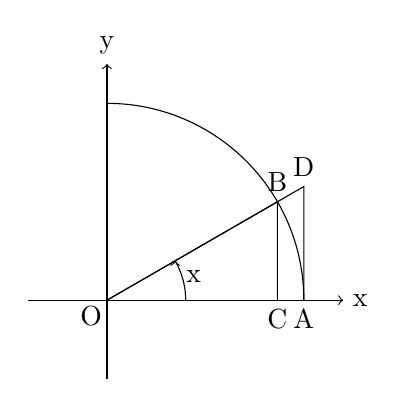
\begin{tikzpicture}[>=to]
        \begin{scope}
            \draw[->] (-1,0)--(3,0)node[right]{x};
            \draw[->] (0,-1)--(0,3)node[above]{y};
            \draw[] (2.5,0) arc(0:90:2.5) (1,2.5);
            \draw[->] (1,0) arc(0:30:1) ({cos (pi/6 r)},{sin (pi/6 r)});
            \draw (0,0)--(30:2.5)node[above]{B}--({(2.5)*(cos (pi/6 r))},0)node[below]{C};
            \draw (0,0)--(2.5,{(2.5)*(tan (pi/6 r))})node[above]{D}--(2.5,0)node[below]{A};
            \node at (-.2,-.2) {O};
            \node at (1.1,.3) {x};
        \end{scope}
    \end{tikzpicture}\\
    \begin{displaymath}
        \begin{split}
            OB&=OA=1\\
            \vartriangle AOB&\leqslant \mbox{扇形面积}\leqslant\vartriangle AOD\\
            \frac{1}{2}\sin x&\leqslant\frac{1}{2}x\leqslant\frac{1}{2}\tan x\\
            \sin x&\leqslant x\leqslant \tan \\
            1&\geqslant\frac{\sin x}{x}\geqslant \cos x\\
            \lim\limits_{x\to 0}1&\geqslant\lim\limits_{x\to 0}\frac{\sin x}{x}\geqslant\lim\limits_{x\to 0}\cos x\\
            1&\geqslant\lim\limits_{x\to 0}\frac{\sin x}{x}\geqslant1\\
            \lim\limits_{x\to 0}\frac{\sin x}{x} &= 1
        \end{split}
    \end{displaymath}
\end{center}

\textbf{\large \ref{limit_1_2}}
\begin{displaymath}
    \begin{split}
        \left|1-\cos x\right|=1-\cos x&=2\sin^2 \frac{x}{2}\\
        &\leqslant 2\left(\frac{x}{2}\right)^2\\
        0\leqslant 1-\cos x &\leqslant \frac{x^2}{2}\\
        \lim\limits_{x\to 0}0\leqslant\lim\limits_{x\to 0}\left(1-\cos x\right)&\leqslant\lim\limits_{x\to 0}{\frac{x^2}{2}}\\
        0\leqslant\lim\limits_{x\to 0}\left(1-\cos x\right)&\leqslant 0\\
        \lim\limits_{x\to 0}\left(1-\cos x\right) &=0\\
        \lim\limits_{x\to 0}\cos x&=1
    \end{split}
\end{displaymath}

\textbf{\large \ref{limit_1_3}}
\begin{displaymath}
    \begin{split}
        \lim\limits_{x\to 0}\frac{\tan x}{x}&=\lim\limits_{x\to 0}\frac{\sin x}{x}\frac{1}{\cos x}\\
        &=\lim\limits_{x\to 0}\frac{\sin x}{x}\lim\limits_{x\to 0}\frac{1}{\cos x}\\
        &=1
    \end{split}
\end{displaymath}

\textbf{\large \ref{limit_1_4}}
\begin{displaymath}
    \begin{split}
        \lim\limits_{x\to 0}\frac{1-\cos x}{\frac{1}{2}x^2}&=\lim\limits_{x\to 0}\frac{2\sin^2\frac{x}{2}}{\frac{1}{2}x^2}\\
        &=\lim\limits_{x\to 0}\left(\frac{\sin \frac{x}{2}}{\frac{x}{2}}\right)^2\\
        &=1
    \end{split}
\end{displaymath}

\textbf{\large \ref{limit_1_5}}
\begin{displaymath}
    \centering
    \begin{split}
        x=\sin t,\ t=\arcsin x\\ 
        x\rightarrow 0,\ t\rightarrow 0\\
        \lim\limits_{x\to 0}\frac{\arcsin x}{x}=\lim\limits_{x\to 0}\frac{t}{\sin t}=1
    \end{split}
\end{displaymath}

\textbf{\large \ref{limit_1_6}}
\begin{displaymath}
    \centering
    \begin{split}
        x=\tan t,\ t=\arctan x\\ 
        x\rightarrow 0,\ t\rightarrow 0\\
        \lim\limits_{x\to 0}\frac{\arctan x}{x}=\lim\limits_{t\to 0}\frac{t}{\tan t}=1
    \end{split}
\end{displaymath}

\textbf{\large \ref{limit_1_7}}
\begin{displaymath}
    \centering
    \begin{split}
        \lim\limits_{x\to 0}\frac{\ln \left(1+x\right)}{x}=\lim\limits_{x\to 0}\ln \left(1+x\right)^\frac{1}{x}=\ln e=1
    \end{split}
\end{displaymath}

\textbf{\large \ref{limit_1_8}}
\begin{displaymath}
    \centering
    \begin{split}
        e^x-1=t,\ x=\ln\left(t+1\right)\\
        x\rightarrow 0,\ t\rightarrow 0\\
        \lim\limits_{x\to 0}\frac{e^x-1}{x}=\lim\limits_{t\to 0}\frac{t}{\ln\left(t+1\right)}=1
    \end{split}
\end{displaymath}

\textbf{\large \ref{limit_1_9}}
\begin{displaymath}
    \centering
    \begin{split}
        \lim\limits_{x\to 0}\frac{\left(1+x\right)^n-1}{nx}=\lim\limits_{x\to 0}\left(\frac{e^{n\ln \left(1+x\right)}-1}{n\ln\left(1+x\right)}\cdot\frac{\ln\left(1+x\right)}{x}\right)=1
    \end{split}
\end{displaymath}

\textbf{\large \ref{limit_2_1}}
\begin{displaymath}
    \centering
    \begin{split}
        x_n&=\left(1+\frac{1}{n}\right)^n=\sum_{m = 0}^{n} C_n^m 1^{n-m}\left(\frac{1}{n}\right)^m=\sum_{m = 0}^{n} C_n^m \left(\frac{1}{n}\right)^m\\
        &=C_n^0\left(\frac{1}{n}\right)^0+C_n^1\left(\frac{1}{n}\right)^1+ \sum_{m = 2}^{n} C_n^m \left(\frac{1}{n}\right)^m\\
        &=1+1+ \sum_{m = 2}^{n} \frac{n!}{m!\left(n-m\right)!} \left(\frac{1}{n}\right)^m\\
        &=1+1+ \sum_{m = 2}^{n} \frac{\overbrace{\left(n\right)\left(n-1\right)\cdots\left(n-m+1\right)}^{m}}{m!} \left(\frac{1}{n}\right)^m\\
        &=1+1+ \sum_{m = 2}^{n} \frac{1}{m!}\left(\frac{n}{n}\right)\left(\frac{n-1}{n}\right)\cdots\left(\frac{n-m+1}{n}\right) \\
        &=1+1+ \sum_{m = 2}^{n} \frac{1}{m!}\left(1-\frac{1}{n}\right)\left(1-\frac{2}{n}\right)\cdots\left(1-\frac{m-1}{n}\right) \\
        x_{n+1}&=1+1+ \sum_{m = 2}^{n+1} \frac{1}{m!}\left(1-\frac{1}{n+1}\right)\left(1-\frac{2}{n+1}\right)\cdots\left(1-\frac{m-1}{n+1}\right) \\
        x_n&<x_{n+1}\qquad\mbox{单调增加}\\
        x_n&<1+1+\frac{1}{2!}+\frac{1}{3!}+\cdots+\frac{1}{n!}\\
        &<1+1+\frac{1}{2^2}+\frac{1}{2^3}+\cdots+\frac{1}{n^2}=1+\frac{1-\left(\frac{1}{2}\right)^2}{1-\frac{1}{2}}\\
        &<1+\frac{1}{1-\frac{1}{2}}\\
        &<3\qquad \mbox{有界}
    \end{split}
\end{displaymath}

\subsection{\centering 第\ref{zhang_derivative}章}
\textbf{\large \ref{derivative_continuity}}
\begin{displaymath}
    \begin{split}
        f'(x_0)&=\lim\limits_{\vartriangle x\to 0}\frac{\vartriangle y}{\vartriangle x}\qquad\mbox{因为极限存在与无穷小的关系}\\
        \frac{\vartriangle y}{\vartriangle x}&=f'(x_0)+\alpha\qquad\alpha \mbox{为}\vartriangle x\to 0\mbox{时的无穷小}\\
        \vartriangle y&=f'(x_0)\vartriangle x+\alpha\vartriangle x\\
        \lim\limits_{\vartriangle x\to 0}\vartriangle y&=\lim\limits_{\vartriangle x\to 0}\left[f'(x_0)\vartriangle x+\alpha\vartriangle x\right]=0\\
        \lim\limits_{x\to x_0}f(x)&=f(x_0)\Leftrightarrow \lim\limits_{\vartriangle x\to 0}\left[f(x_0+\vartriangle x)-f(x_0)=0\right]\Leftrightarrow\lim\limits_{\vartriangle x\to 0}\vartriangle y=0 \\
    \end{split}
\end{displaymath}

\textbf{\large \ref{derivative_1}}
\begin{displaymath}
    \begin{split}
        (C)'&=\lim\limits_{\vartriangle x\to 0}\frac{f(x_0+\vartriangle x)-f(x_0)}{\vartriangle x}\\
        &=\lim\limits_{\vartriangle x\to 0} \frac{C-C}{\vartriangle x}\\
        &=0
    \end{split}
\end{displaymath}

\textbf{\large \ref{derivative_2}}
\begin{displaymath}
    \begin{split}
        \left(x^a\right)'&=\lim\limits_{x\to x_0}\frac{f(x)-f(x_0)}{x-x_0}\\
        &=\frac{x^a-x_0^a}{x-x_0}\\
        &=\frac{(x-x_0)\left(x^{a-1}+x^{a-2}x_0+\cdots+xx_0^{a-2}+x_0^{a-1}\right)}{x-x_0}\\
        &=ax_0^{a-1}
    \end{split}
\end{displaymath}

\textbf{\large \ref{derivative_3}}
\begin{displaymath}
    \begin{split}
        \left(a^x\right)'&=\lim\limits_{\vartriangle x\to 0}\frac{a^{x+\vartriangle x}-a^x}{\vartriangle x}\\
        &=a^x\lim\limits_{\vartriangle x\to 0}\frac{a^{\vartriangle x}-1}{\vartriangle x}\\
        &=a^x\lim\limits_{\vartriangle x\to 0}\frac{e^{\vartriangle x \ln a}-1}{\vartriangle x}\\
        &=a^x\ln a
    \end{split}
\end{displaymath}

\textbf{\large \ref{derivative_4}}
\begin{displaymath}
    \begin{split}
        \left(e^x\right)'=e^x\ln e=e^x
    \end{split}
\end{displaymath}

\textbf{\large \ref{derivative_5}}
\begin{displaymath}
    \begin{split}
        \left(\log_a^x\right)'&=\lim\limits_{\vartriangle x\to 0}\frac{\log_a^{x+\vartriangle x}-\log_a^x}{\vartriangle x}\\
        &=\lim\limits_{\vartriangle x\to 0}\frac{\log_a^{1+\frac{\vartriangle x}{x}}}{\vartriangle x}\\
        &=\lim\limits_{\vartriangle x\to 0}\frac{\ln{1+\frac{\vartriangle x}{x}}}{\ln a\vartriangle x}\\
        &=\frac{1}{\ln a}\lim\limits_{\vartriangle x\to 0}\frac{\frac{\vartriangle x}{x}}{\vartriangle x}\\
        &=\frac{1}{x\ln a}
    \end{split}
\end{displaymath}

\textbf{\large \ref{derivative_6}}
\begin{displaymath}
    \begin{split}
        \left(\ln^x\right)'&=\frac{1}{x\ln e}\\
        &=\frac{1}{x}
    \end{split}
\end{displaymath}

\textbf{\large \ref{derivative_sin}}
\begin{displaymath}
    \begin{split}
        (\sin x)'&=\lim\limits_{\vartriangle x\to 0}\frac{\sin (x_0 +\vartriangle x)-\sin x_0}{\vartriangle x}\\
        &=\lim\limits_{\vartriangle x\to 0}\frac{2\cos(x_0+\frac{\vartriangle x}{2})\sin \frac{\vartriangle x}{2}}{\vartriangle x}\\
        &=\lim\limits_{\vartriangle x\to 0}\cos(x_0+\frac{\vartriangle x}{2})\frac{\sin\frac{\vartriangle x}{2}}{\frac{\vartriangle x}{2}}\\
        &=cos x_0
    \end{split}
\end{displaymath}

\textbf{\large \ref{derivative_arcsin}}
\begin{displaymath}
    \begin{split}
        (\arcsin x)'=\frac{1}{\frac{dx}{\mathrm{d}{y}}}&=\frac{1}{\frac{d\sin y}{\mathrm{d}{y}}}\\
        &=\frac{1}{\cos y}\\
        &=\frac{1}{\sqrt{1-\sin^2 y}}\\
        &=\frac{1}{\sqrt{1-x^2}}
    \end{split}
\end{displaymath}

\textbf{\large \ref{derivative_csc}}
\begin{displaymath}
    \begin{split}
        (\csc x)'=(\frac{1}{\sin x})‘&=\frac{(1)'\cdot sin x-(\sin x)'\cdot 1}{\sin^2x}\\
        &=\frac{-\cos x}{\sin^2x}\\
        &=-\csc x\cdot\cot x
    \end{split}
\end{displaymath}

\textbf{\large \ref{derivative_cos}}
\begin{displaymath}
    \begin{split}
        (\cos x)'&=\lim\limits_{\vartriangle x\to 0}\frac{\cos(x_0+\vartriangle x)-cos(x_0)}{\vartriangle x}\\
        &=\lim\limits_{\vartriangle x\to 0}\frac{-2\sin \left(x_0+\frac{\vartriangle x}{2}\right)\sin\frac{\vartriangle x}{2}}{\vartriangle x}\\
        &=\lim\limits_{\vartriangle x\to 0}-\sin \left(x_0+\frac{\vartriangle x}{2}\right)\frac{\sin\frac{\vartriangle x}{2}}{\frac{\vartriangle x}{2}}\\
        &=-\sin x
    \end{split}
\end{displaymath}

\textbf{\large \ref{derivative_arccos}}
\begin{displaymath}
    \begin{split}
        (\arccos x)'=\frac{1}{\frac{dx}{\mathrm{d}{y}}}&=\frac{1}{\frac{d\cos y}{\mathrm{d}{y}}}\\
        &=\frac{1}{-\sin y}\\
        &=-\frac{1}{\sqrt{1-\cos^2 y}}\\
        &=-\frac{1}{\sqrt{1-x^2}}
    \end{split}
\end{displaymath}

\textbf{\large \ref{derivative_sec}}
\begin{displaymath}
    \begin{split}
        (\sec x)'=\left(\frac{1}{\cos x}\right)'&=\frac{(1)'\cdot\cos x-(\cos x)'\cdot 1}{\cos^2x}\\
        &=\frac{\sin x}{\cos^2x}\\
        &=\sec x\cdot\tan x
    \end{split}
\end{displaymath}

\textbf{\large \ref{derivative_tan}}
\begin{displaymath}
    \begin{split}
        (\tan x)'=\left(\frac{\sin x}{\cos x}\right)'&=\frac{(\sin x)'\cos x-(\cos x)'\sin x}{\cos^2x}\\
        &=\frac{\cos^2 x+\sin^2 x}{\cos^2x}\\
        &=\sec^2 x
    \end{split}
\end{displaymath}

\textbf{\large \ref{derivative_arctan}}
\begin{displaymath}
    \begin{split}
        (\arctan x)'=\frac{1}{\frac{dx}{\mathrm{d}{y}}}&=\frac{1}{\frac{d\tan y}{\mathrm{d}{y}}}\\
        &=\frac{1}{\sec y}\\
        &=\frac{1}{1+\tan^2 y}\\
        &=\frac{1}{1+x^2}
    \end{split}
\end{displaymath}

\textbf{\large \ref{derivative_cot}}
\begin{displaymath}
    \begin{split}
        (\cot x)'=\left(\frac{\cos x}{\sin x}\right)'&=\frac{(\cos x)'\sin x-(\sin x)'\cos x}{\sin^2x}\\
        &=-\frac{\sin^2 x+\cos^2 x}{\cos^2x}\\
        &=-\csc^2 x
    \end{split}
\end{displaymath}

\textbf{\large \ref{derivative_arccot}}
\begin{displaymath}
    \begin{split}
        (\operatorname{arccot}{x})'=\frac{1}{\frac{dx}{\mathrm{d}{y}}}&=\frac{1}{\frac{d\cot y}{\mathrm{d}{y}}}\\
        &=\frac{1}{-\csc^2 y}\\
        &=-\frac{1}{1+\cot^2 y}\\
        &=-\frac{1}{1+x^2}
    \end{split}
\end{displaymath}

\textbf{\large \ref{derivative_sinh}}
\begin{displaymath}
    \begin{split}
        (\sinh x)'&=\left(\frac{e^x-e^{-x}}{2}\right)'\\
                                    &=\frac{e^x+e^{-x}}{2}\\
                                    &=\cosh x
    \end{split}
\end{displaymath}
\textbf{\large \ref{derivative_cosh}}
\begin{displaymath}
    \begin{split}
        (\cosh x)'&=\left(\frac{e^x+e^{-x}}{2}\right)'\\
                                    &=\frac{e^x-e^{-x}}{2}\\
                                    &=\sinh x
    \end{split}
\end{displaymath}

\textbf{\large \ref{derivative_tanh}}
\begin{displaymath}
    \begin{split}
        (\tanh x)'&=\left(\frac{e^x-e^{-x}}{e^x+e^{-x}}\right)'\\
                                    &=\frac{\frac{d(e^x-e^{-x})}{\mathrm{d}{x}}(e^x+e^{-x})-\frac{d(e^x+e^{-x})}{\mathrm{d}{x}}(e^x-e^{-x})}{\left(e^x+e^{-x}\right)^2}\\
                                    &=\frac{\left(e^x+e^{-x}\right)^2-\left(e^x-e^{-x}\right)^2}{\left(e^x+e^{-x}\right)^2}\\
                                    &=\frac{2^2}{\left(e^x+e^{-x}\right)^2}\\
                                    &=\frac{1}{\cosh^2 x}
                                \end{split}
\end{displaymath}

\textbf{\large \ref{derivative_arcsinh}}
\begin{displaymath}
    \begin{split}
        (\operatorname{arcsinh}{x})' &=\left[\ln(x+\sqrt{x^2+1})\right]'\\
                                    &=\frac{d \ln(x+\sqrt{x^2+1})}{\mathrm{d}{\left(x+\sqrt{x^2+1}\right)}}\cdot\frac{d \left(x+\sqrt{x^2+1}\right)}{\mathrm{d}{x}}\\
                                    &=\frac{1}{x+\sqrt{x^2+1}}\cdot\left(\frac{dx}{dx}+\frac{d \left(\sqrt{x^2+1}\right)}{d\left(x^2+1\right)}\cdot\frac{d(x^2+1)}{dx}\right)\\
                                    &=\frac{1}{x+\sqrt{x^2+1}}\cdot\left(1+\frac{1}{2\sqrt{x^2+1}}\cdot 2x\right)\\                                    
                                    &=\frac{1}{x+\sqrt{x^2+1}}\cdot\frac{x+\sqrt{x^2+1}}{\sqrt{x^2+1}}\\
                                    &=\frac{1}{\sqrt{x^2+1}}
                                \end{split}
\end{displaymath}

\textbf{\large \ref{derivative_arccosh}}
\begin{displaymath}
    \begin{split}
        (\operatorname{arccosh}{x})' &=\left[\ln(x+\sqrt{x^2-1})\right]'\\
                                    &=\frac{d \ln(x+\sqrt{x^2-1})}{\mathrm{d}{\left(x+\sqrt{x^2-1}\right)}}\cdot\frac{d \left(x+\sqrt{x^2-1}\right)}{\mathrm{d}{x}}\\
                                    &=\frac{1}{x+\sqrt{x^2-1}}\cdot\left(\frac{dx}{dx}+\frac{d \left(\sqrt{x^2-1}\right)}{d\left(x^2-1\right)}\cdot\frac{d(x^2-1)}{dx}\right)\\
                                    &=\frac{1}{x+\sqrt{x^2-1}}\cdot\left(1+\frac{1}{2\sqrt{x^2-1}}\cdot 2x\right)\\                                    
                                    &=\frac{1}{x+\sqrt{x^2-1}}\cdot\frac{x+\sqrt{x^2-1}}{\sqrt{x^2-1}}\\
                                    &=\frac{1}{\sqrt{x^2-1}}
                                \end{split}
\end{displaymath}

\textbf{\large \ref{derivative_arctanh}}
\begin{displaymath}
    \begin{split}
        (\operatorname{arctanh}{x})' &=\left[\frac{1}{2}\ln(\frac{1+x}{1-x})\right]'\\
        &=\frac{1}{2}\cdot\frac{d\left[\ln(\frac{1+x}{1-x})\right]}{\mathrm{d}{\left(\frac{1+x}{1-x}\right)}}\cdot\frac{d\left(\frac{1+x}{1-x}\right)}{\mathrm{d}{x}}\\
        &=\frac{1}{2}\cdot\frac{1}{\left(\frac{1+x}{1-x}\right)}\cdot\frac{\frac{d(1+x)}{\mathrm{d}{x}}(1-x)-\frac{d(1-x)}{\mathrm{d}{x}}(1+x)}{(1-x)^2}\\
        &=\frac{1}{2}\cdot\frac{1-x}{1+x}\cdot\frac{(1-x)+(1+x)}{(1-x)^2}\\
        &=\frac{1}{(1+x)(1-x)}\\
        &=\frac{1}{1-x^2}
    \end{split}
\end{displaymath}

\textbf{\large \ref{limit_operation_1}}
\begin{displaymath}
    \begin{split}
        \left[Cu(x)\right]'&=\lim\limits_{\vartriangle x\to 0}\frac{Cu(x+\vartriangle x)-Cu(x)}{\vartriangle x}\\
        &=C\lim\limits_{\vartriangle x\to 0}\frac{u(x+\vartriangle x)-u(x)}{\vartriangle x}\\
        &=Cu'(x)
    \end{split}
\end{displaymath}
\textbf{\large \ref{limit_operation_2}}
\begin{displaymath}
    \begin{split}
            (u(x)\pm v(x))'&=\lim\limits_{\vartriangle x\to 0}\frac{u(x+\vartriangle x)-u(x)\pm v(x+\vartriangle x)-v(x)}{\vartriangle x}\\
        &=\lim\limits_{\vartriangle x\to 0}\frac{u(x+\vartriangle x)-u(x)}{\vartriangle x}\pm\lim\limits_{\vartriangle x\to 0}\frac{v(x+\vartriangle x)-v(x)}{\vartriangle x}\\
        &=u'(x)\pm v'(x)
    \end{split}
\end{displaymath}
\textbf{\large \ref{limit_operation_3}}
\begin{displaymath}
    \begin{split}
        \left[u(x)\cdot v(x)\right]'&=\lim\limits_{\vartriangle x\to 0}\frac{u(x+\vartriangle x)v(x+\vartriangle x)-u(x)v(x)-u(x)v(x+\vartriangle x)+u(x)v(x+\vartriangle x)}{\vartriangle x}\\
            &=\lim\limits_{\vartriangle x\to 0}\frac{\left[u(x+\vartriangle x)-u(x)\right]v(x+\vartriangle x)+u(x)\left[v(x+\vartriangle x)-v(x)\right]}{\vartriangle x}\\
            &=u'(x)\lim\limits_{\vartriangle x\to 0}v(x+\vartriangle x)+u(x)v'(x)\\
            &=u'(x)v(x)+v'(x)u(x)
    \end{split}
\end{displaymath}
\textbf{\large \ref{derivative_of_inverse_function}}
\begin{displaymath}
    \begin{split}
        \left[f^{-1}(y)\right]'|_{y=y_0}&=\lim\limits_{y\to y_o}\frac{f^{-1}(y)-f^{-1}(y_0)}{y-y_0}\\
        &=\lim\limits_{y\to y_o}\frac{x-x_0}{y-y_0}\\
        &=\lim\limits_{x\to x_o}\frac{x-x_0}{f(x)-f(x_0)}\\
        &=\lim\limits_{x\to x_o}\frac{1}{\frac{f(x)-f(x_0)}{x-x_0}}\\
        &=\frac{1}{f'(x)}\\
    \end{split}
\end{displaymath}

\textbf{\large \ref{derivative_of_composite_functions}}
\begin{displaymath}
    \begin{split}
        \mbox{定义函数}\quad A(u)&=\begin{cases}
            \frac{f(u)-f(u_0)}{u-u_0}. &u\neq u_0\\
            f'(u_0),&u= u_0
        \end{cases}\\
        A(u)\mbox{在}u_o&\mbox{处连续,既有}\\
        \lim\limits_{u\to u_o}A(u)&=A(u_0)=f'(u_0)\\
        \mbox{由恒等式}f(u)-f(u_0)&=A(u)(u-u_0)\mbox{我们有}\\
        \frac{F(x)-F(x_0)}{x-x_0}&=\frac{f\left[g(x)\right]-f\left[g(x_0)\right]}{x-x_0}\\
        &=A\left[g(x)\right]\frac{g(x)-g(x_0)}{x-x_0}\\
        \lim\limits_{x\to x_0}\frac{F(x)-F(x_0)}{x-x_0}&=\lim\limits_{x\to x_0}A\left[g(x)\right]\frac{g(x)-g(x_0)}{x-x_0}\\
        F'(x_0)&=f'(g(x_0))g'(x_0)
    \end{split}
\end{displaymath}

\subsection{\centering 第\ref{zhang_differential}章}
\textbf{\large \ref{differential_to_derivative}}
\begin{displaymath}
    \begin{split}
            \vartriangle y&=A\vartriangle x+\circ(\vartriangle x)\\
            \frac{\vartriangle y}{\vartriangle x}&=A+\frac{\circ(\vartriangle x)}{\vartriangle x}\\
            \lim\limits_{\vartriangle x\to 0}\frac{\vartriangle y}{\vartriangle x}&=\lim\limits_{\vartriangle x\to 0}\left[A+\frac{\circ(\vartriangle x)}{\vartriangle x}\right]\\
            f'(x_0)&=A+0\\
            f'(x_0)&=A
        \end{split}
\end{displaymath}
\textbf{\large \ref{derivative_to_differential}}
\begin{center}
            $\mbox{设}f(x)\mbox{在}x_0\mbox{点可导},f'(x_0)=\lim\limits_{\vartriangle x \to 0}\frac{\vartriangle y}{\vartriangle x}\mbox{存在}$\\
            $\left(\mbox{极限与无穷小的关系:}\lim f(x)=A\Leftrightarrow f(x)=A+\alpha\right)$\\
            $\frac{\vartriangle y}{\vartriangle x}=f'(x_0)+\alpha$\\
            $\vartriangle y=f'(x_0)\vartriangle x+\alpha \vartriangle x$\\
            $\mbox{其中}\alpha \mbox{为}\vartriangle x\to 0\mbox{时的无穷小。}$\\
            $\lim\limits_{\vartriangle x\to 0}\frac{\alpha \vartriangle x}{\vartriangle x}=\lim\limits_{\vartheta x\to 0}\alpha = 0$\\
            $\alpha \vartriangle x=\circ(\vartriangle x)$\\
            $\vartriangle y=f'(x_0)\vartriangle x+\circ(\vartriangle x)$
\end{center}

\textbf{\large \ref{differential_operation_rule_1}}
\begin{displaymath}
    \begin{split}
        d(u\pm v)&=(u\pm v)'dx\\
                &=(u)'dx \pm (v')dx\\
                &=du\pm dv
    \end{split}
\end{displaymath}

\textbf{\large \ref{differential_operation_rule_2}}
\begin{displaymath}
    \begin{split}
        d(u\cdot v)&=(u\cdot v)'dx\\
                &=(u)'vdx - (v')udx\\
                &=vdu - udv
    \end{split}
\end{displaymath}

\textbf{\large \ref{differential_operation_rule_3}}
\begin{displaymath}
    \begin{split}
        d\left(\frac{u}{v}\right)&=\left(\frac{u}{v}\right)'dx\\
                &=\frac{(u)'v - (v')u}{v^2}dx\\
                &=\frac{vdu - udv}{v^2}
    \end{split}
\end{displaymath}

\textbf{\large \ref{Fermat_Lemma}}
\begin{center}
    $\lim\limits_{\vartriangle x\to 0}\frac{f(x_0+\vartriangle x)}{\vartriangle x}=f'(x_0)$\\
    $f(x_0+\vartriangle x)-f(x_0)\leqslant 0$\\
    $\begin{cases}
        \vartriangle x>0\begin{cases}
            \frac{f(x_0+\vartriangle x)-f(x_0)}{\vartriangle x}\leqslant 0\Rightarrow f'(x_0^+) =\lim\limits_{\vartriangle x \to 0}\frac{f(x_0+\vartriangle x)-f(x_0)}{\vartriangle x}\leqslant 0
        \end{cases}\\
        \vartriangle x<0\begin{cases}
            \frac{f(x_0+\vartriangle x)-f(x_0)}{\vartriangle x}\geqslant 0\Rightarrow f'(x_0^-) =\lim\limits_{\vartriangle x \to 0}\frac{f(x_0+\vartriangle x)-f(x_0)}{\vartriangle x}\geqslant 0
        \end{cases}
    \end{cases}$\\
    $f'(x_0)=f'(x_0^+)=f'(x_0^-)\Rightarrow f'(x_0)= 0$
\end{center}

\textbf{\large \ref{Rolle's theorem}}
\begin{center}
    $M=\max\{f(x)|x\in[a,b]\},m=\min\{f(x)|x\in[a,b]\}$
    $\begin{cases}
        M=m\Rightarrow M=m=f(a)=f(b),\mbox{此时}f(x)\mbox{为常数},\forall \xi \in(a,b),f'(\xi)=0\\
        M>m \begin{cases}
            f(a)>m \Rightarrow \exists \xi \in(a,b),f(\xi)=m,\mbox{根据费马引理},f'(\xi)=0\\
            f(a)<M5 \Rightarrow \exists \xi \in(a,b),f(\xi)=M,\mbox{根据费马引理},f'(\xi)=0\\
        \end{cases}
    \end{cases}$
\end{center}
\textbf{\large \ref{Lagrange's theorem}}
\begin{displaymath}
    \begin{split}
        \varphi(x)&=f(x)-\frac{f(b)-f(a)}{b-a}x\\
        \varphi(a)&=f(a)-\frac{f(b)-f(a)}{b-a}a=\frac{bf(a)-af(b)}{b-a}\\
        \varphi(b)&=f(b)-\frac{f(b)-f(a)}{b-a}b=\frac{bf(a)-af(b)}{b-a}\\
        \varphi(a)&=\varphi(b),\exists \xi\in(a,b),\varphi'(\xi)=0\\
        f'(\xi)&=\frac{f(b)-f(a)}{b-a}\\
        f'(\xi)(b-a)&7=f(b)-f(a)
    \end{split}
\end{displaymath}

\textbf{\large \ref{cauchy_theorem}}
\begin{displaymath}
    \begin{split}
        \varphi(x)&=f(x)-\frac{f(b)-f(a)}{F(b)-F(a)}\left[F(x)-F(a)\right] \\
        \varphi(a)&=\varphi(b)=f(a)\\
        \varphi'(\xi)&=0\\
        f'(\xi)&=\frac{f(b)-f(a)}{F(b)-F(a)}F'(\xi)\\
        \frac{f'(\xi)}{F'(\xi)}&=\frac{f(b)-f(a)}{F(b)-F(a)}
    \end{split}
\end{displaymath}

\textbf{\large \ref{l'hospital rule}}
    \begin{center}
        $f(x),F(x)\mbox{的去心邻域可导,}\lim\limits_{x\to x_0}\frac{f(x)}{F(x)}\mbox{与}f(x_0),F(x_0)\mbox{无关。规定}f(x_0)=0,F(x_0)=0$\\
$\mbox{此时}\lim\limits_{x\to x_0}f(x)=0=f(x_0)\quad\lim\limits_{x\to x_0}F(x)=0=F(x_0)\quad\mbox{此时在$x_0$点处也连续}$\\
    \end{center}
    \begin{displaymath}
        \begin{split}
    \frac{f(x)}{F(x)}&=\frac{f(x)-f(x_0)}{F(x)-F(x_0)}=\frac{f'(\xi)}{F'(\xi)}\\
    \lim\limits_{x\to x_0}\frac{f(x)}{F(x)}&=\lim\limits_{x\to x_0}\frac{f'(\xi)}{F'(\xi)}\\
    x\rightarrow x_0,&\mbox{时}\xi\rightarrow x_0\qquad \mbox{符号$\xi$换成x}\\
    \lim\limits_{x\to x_0}\frac{f(x)}{F(x)}&=\lim\limits_{\xi\to x_0}\frac{f'(\xi)}{F'(\xi)}=\lim\limits_{x\to x_0}\frac{f'(x)}{F'(x)}
        \end{split}
    \end{displaymath}

\textbf{\large \ref{lagrange_remainder}}
\begin{displaymath}
    \begin{split}
        \frac{R_n(x)}{(x-x_0)^{n+1}}&=\frac{R_n(x)-R_n(x_0)}{(x-x_0)^{n+1}-(x_0-x_0)^{n+1}}=\frac{R_n'(\xi_1)}{(n+1)(\xi_1-x_0)^n}\\
        \frac{1}{n+1}\cdot\frac{R_n'(\xi_1)}{(\xi_2-x_0)^n}&=\frac{1}{n+1}\cdot\frac{R_n'(\xi_1)-R_n'(x_0)}{(\xi_1-x_0)^{n}-(x_0-x_0)^{n}}=\frac{1}{n+1}\cdot\frac{R_n''(\xi_2)}{(n)(\xi_2-x_0)^{n-1}}\\
        &\vdots\\
        \frac{R_n^{(n)}(\xi_n)}{(n+1)!(\xi_n-x_0)}&=\frac{R_n^{(n)}(\xi_n)-R_n^{(n)}(x_0)}{(n+1)!(\xi_n-x_0)-0}=\frac{R_n^{(n+1)}(\xi)}{(n+1)!}\\
        \frac{R_n^{(n+1)}(\xi)}{(n+1)!}&=\frac{f^{(n+1)}(\xi)-P_n^{(n+1)}(\xi)}{(n+1)!}=\frac{f^{(n+1)}(\xi)}{(n+1)!}\\
        R_n(x)&=\frac{f^{(n+1)}(\xi)}{(n+1)!}(x-x_0)^{n+1}
\end{split}
\end{displaymath}
\centerline{$\xi_1\in(x,x_0),\xi_2\in(\xi_1,x_0),\xi_n\in(\xi_{n-1},x_0),\xi\in(\xi_n,x_0)$}

\textbf{\large \ref{Piano_remainder}}
\begin{displaymath}
    \begin{split}
      \lim\limits_{x\to x_0}\frac{R_n(x)}{(x-x_0)^n}&=\lim\limits_{x\to x_0}\frac{R_n'(x)}{n(x-x_0)^{n-1}}\\
      &=\lim\limits_{x\to x_0}\frac{R_n''(x)}{n(n-1)(x-x_0)^{n-2}}\\
      &=\lim\limits_{x\to x_0}\frac{R_n^{(n)}(x)}{n!}\\
      &=\frac{1}{n}\cdot 0\\
      &=0
\end{split}
\end{displaymath}
 %证明
\end{document}